% Bremen Big Data Challenge - Edition 2019
%
% Data Analysis Competition
%
% Team `gentleman`
%
% Created on March 10, 2019
%
% Authors:
%   Gari Ciodaro <g.ciodaroguerra@jacobs-university.de>
%   Diogo Cosin <d.ayresdeoliveira@jacobs-university.de>
%   Ralph Florent <r.florent@jacobs-university.de>
%
% Contents block for the documentation
%
% 1) Introduction
% 2) Background of the data (data description)
% 3) Data preprocessing
% 4) Data exploitation
% 5) Data Analysis
% 6) Conclusion / Results
% 7) References / Bibliography

% ==============================================================================
% START: Methods, Results, Discussions, Conclusion
% ==============================================================================

\section{Background of the Data}
\subsection{Data Source}

Provided by \emph{"The Bremen Big Data Challenge 2019" Organizers}, the collected data are based on
daily athletic movements \parencite{bbdc}. Using wearable sensors above and below the knee (See
Figure \ref{fig:sensor-placement}) of the individual (athletic), a dataset of 19 individuals, mainly
identified as \emph{subjects}, has been recorded. And as the competition requires, the data of 15
out of the total number of subjects are used as the training dataset and the remaining part as the
testing dataset. The dataset is publicly available online on the official website:
\href{https://bbdc.csl.uni-bremen.de/images/2019/bbdc_2019_Bewegungsdaten_mit_referenz.zip}{BBDC} or
by simply browsing through the following URL: \emph{https://bbdc.csl.uni-bremen.de/index.php/2019h/28-aufgabenstellung-2019}.

\begin{figure}
    \centering
    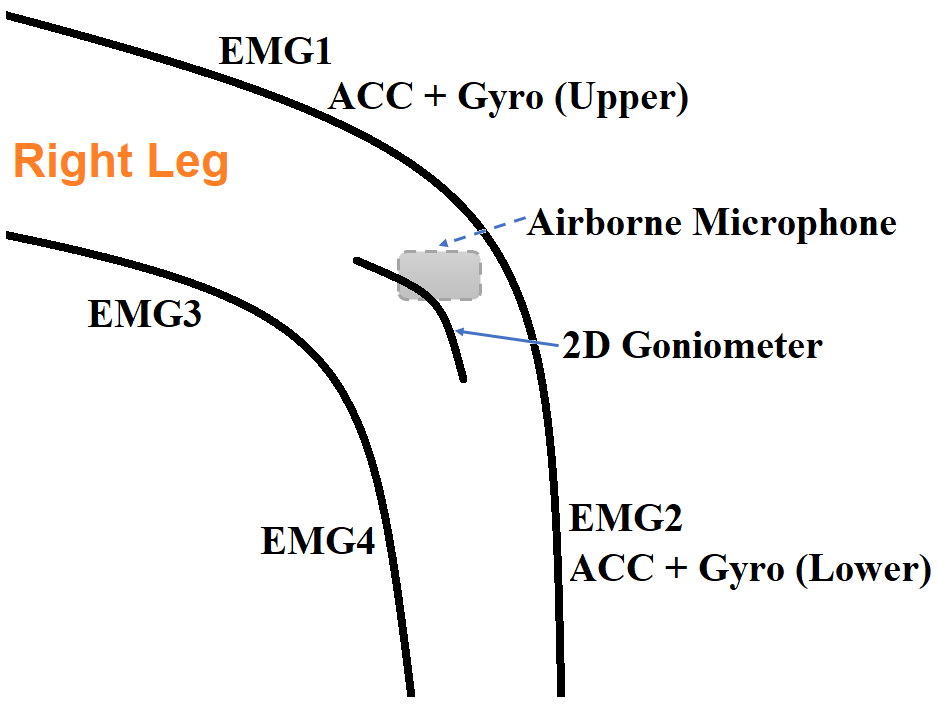
\includegraphics[scale=0.33]{sensor-placement.png}
    \caption{Wearable sensor placement for data measurements. \\ (source: part of the provided data)}
    \label{fig:sensor-placement}
\end{figure}

\subsection{Description and Format}

The data comprise the following 22 movements:
\begin{itemize}
    \item Race ('run')
    \item Walking ('walk')
    \item Standing (standing)
    \item Sitting ('sit')
    \item Get up and sit down ('sit-to-stand', 'stand-to-sit')
    \item Up and down stairs ('stair-up', 'stair-down')
    \item Jump on one or both legs ('jump-one-leg', 'jump-two-leg')
    \item Run left or right ('curve-left-step', 'curve-right-step')
    \item Turn left or right on the spot, left or right foot first ('curve-left-spin-Lfirst',
    'curve-left-spin-Rfirst', 'curve-right-spin-Lfirst', 'curve-right- spin-Rfirst ')
    \item Lateral steps to the left or right ('lateral-shuffle-left', 'lateral-shuffle-right')
    \item Change of direction when running to the right or left, left or right foot first
    ('v-cut-left-left', 'v-cut-left-right', 'v-cut-right-left', 'v-cut' right-Rfirst ')
\end{itemize}

The entire data are available as CSV files, or Comma-Separated Values, and partitioned as training and
testing data, respectively represented by the "\textbf{\emph{train.csv}}" and the "\textbf{\emph{challenge.csv}}"
files. Starting with the training dataset file (\textbf{\emph{train.csv}}), it contains
\emph{UTF-8}\footnote{Unicode Transformation Format, extended ASCII, variable-width encoding.}
character-encoded, line-wise plain texts, whose first line identifies the feature names
followed by the feature values. This file contains a total of 6402 lines, which include both the
feature names and the feature values. The feature names are \textit{Subjects}, \textit{Datafile}, \textit{Label},
and the feature values map respectively each feature name. For instance, the first feature values of
the file are: \textit{Subject02}, \textit{ \path{Subject02 / Subject02_Aufnahme002.csv}},
\textit{stand-to-sit}. Table \ref{table:train-data} illustrates a lightweight version of the
data partition of the training dataset file.

\begin{table}
    \begin{center}
        \begin{tabular}{||c | c | c||}
            \hline % Table headers
            \textbf{Subjects} & \textbf{Datafile} & \textbf{Label} \\ [0.5ex]
            \hline \hline % Table body (row-wise contents)
            Subject02 & \path{Subject02 / Subject02_Aufnahme000.csv} & \textit{curve-left-step} \\
            \hline
            Subject02 & \path{Subject02 / Subject02_Aufnahme001.csv} & \textit{curve-left-step} \\
            \hline
            Subject02 & \path{Subject02 / Subject02_Aufnahme002.csv} & \textit{stand-to-sit} \\
            \hline
            ... & ... & ... \\
            \hline
            Subject19 & \path{Subject19 / Subject19_Aufnahme438.csv} & \textit{curve-right-step} \\
            \hline
            Subject19 & \path{Subject19 / Subject19_Aufnahme439.csv} & \textit{curve-right-spin-Rfirst} \\
            \hline
        \end{tabular}
        \caption{Tabular visualization of the "\textbf{\emph{train.csv}}" dataset}
        \label{table:train-data}
    \end{center}
\end{table}

Similarly, the testing dataset file (\textbf{\emph{challenge.csv}}) is formatted using the same structure
with the exception of the \textit{Label} column, which is unknown and marked with an \emph{X}.
The datafile contains a total of 1739 lines counting both the feature names and feature values.
Table \ref{table:test-data} displays a lightweight version of the data partition of the testing
dataset file.

\begin{table}
    \begin{center}
        \begin{tabular}{||c | c | c||}
            \hline % Table headers
            \textbf{Subjects} & \textbf{Datafile} & \textbf{Label} \\ [0.5ex]
            \hline \hline % Table body (row-wise contents)
            Subject01 & \path{Subject01 / Subject01_Aufnahme000.csv} & \textit{X} \\
            \hline
            Subject01 & \path{Subject01 / Subject01_Aufnahme001.csv} & \textit{X} \\
            \hline
            Subject01 & \path{Subject01 / Subject01_Aufnahme002.csv} & \textit{X} \\
            \hline
            ... & ... & ... \\
            \hline
            Subject15 & \path{Subject15 / Subject15_Aufnahme438.csv} & \textit{X} \\
            \hline
            Subject15 & \path{Subject15 / Subject15_Aufnahme439.csv} & \textit{X} \\
            \hline
        \end{tabular}
        \caption{Tabular visualization of the "\textbf{\emph{challenge.csv}}" dataset}
        \label{table:test-data}
    \end{center}
\end{table}

\noindent
\textbf{Important}: Recalling that the dataset is divided into training and testing data, the subjects
"\emph{Subject01, Subject10, Subject14, Subject15}" are the selected ones that are used as testing
data to assess the solutions. Note the difference in the starting and ending rows of Tables
\ref{table:train-data} and \ref{table:test-data}.

As observed in both Tables \ref{table:train-data} and \ref{table:test-data}, each line corresponds
to a recording of a movement. The columns have the following meanings:
\begin{itemize}
    \item \textbf{\emph{Subject}}: The ID of the subject
    \item \textbf{\emph{Datafile}}: Path of the file containing the sensor data for this recording. For each subject,
    there is a folder in which individual data files contain the sensor data for individual motion
    recordings.
    \item \textbf{\emph{Label}}: The movement that was recorded
\end{itemize}

Particularly, the \emph{Label} column of the testing dataset contains repeatedly the letter "\textit{X}"
to indicate that this value is not present. That is, at the time of submitting solutions, the submission should
exactly match the testing data, where each \emph{X} will be replaced by a label. This label corresponds to the
classification result of a specific movement. It is important that the spelling (including upper / lower
case) of the textual labels matches exactly the spelling of the labels in the training data.

As mentioned above, the datafiles are references to other CSV files. For example, the path file
\path{Subject02 / Subject02_Aufnahme000.csv} is a CSV file within a folder named \emph{Subject02}
located in the root path (i.e., the current directory of the downloaded zip files). The CSV file itself
is a dataset with a proper format. Basically, the file has a set of comma-separated numbered-values
that looks like this: \textit{32688, 32224, 32991, 32609,32790,33048, 37168, 34610, 27374, 29068, 29264,
28408, 31784, 28133, 29295, 29244, 33216, 37140, 34736}.

Each line has 19 values (numbers) and represents the sensor values measured at one time (sampled at
1000 Hz). In other words, the columns represent the individual wearable sensors recording the human
activities (see Figure \ref{fig:sensor-placement}):

\begin{center}
    \begin{tabular}{ c c c c c }
     EMG1 & Airborne    & Goniometer X & Goniometer Y & Gyro lower X \\
     EMG2 & ACC upper X & ACC lower X  & Gyro upper X & Gyro lower Y \\
     EMG3 & ACC upper Y & ACC lower Y  & Gyro upper Y & Gyro lower Z \\
     EMG4 & ACC upper Z & ACC lower Z  & Gyro upper Z &
    \end{tabular}
\end{center}


% source is needed
The size of the CSV datafiles varies inappropriately. That is, in most cases, due to inaccurate measurements,
random initialization states, mechanical flaws, computational and processing cost, and so on.


\section{General Comments}

\subsection{Notation} \label{notation}
Let us defined a modeling procedure as  a function $\mathcal{P}(\Theta): \mathbb{R}^{m} \longrightarrow \mathbb{R}^{k}$ where $m$ is the number of features, $k$ is the number of classes, and $\Theta : \{Preprocessing_{method}, Feature_{extration}, Statistical_{Tecnique} \}$ is a set representing parameters. Giving this abstraction $\Theta$ modifies the structure  $\mathcal{P}$ but always takes a \textit{feature vector} $X \in  \mathbb{R}^{m}$, and returns a \textit{Probability vector} $Y \in  \mathbb{R}^{k}$ where each component $\in  [0,1]$.\\

It is clear that the $\mathcal{P}(\Theta)$ that represents exactly the reality regarding athletics movements is unknown to us, which let us to defined a measure of the amount of veracity that a giving $\mathcal{P}$ has compare to reality.

\begin{equation}
accuracy=  \frac{\sum Correct_{classification}}{N}
\end{equation}

\subsection{Cross Validation}

Given the modeling procedure $\mathcal{P}$ defined in the Subsection \ref{notation}
for a given learning task, one usually seeks to evaluate its performance in the
so-called training data and testing data. The training data is not but the set of
data points utilized during the training procedure whereas the testing data is a
completely new data points set. Ideally, an efficient modeling procedure
$\mathcal{P}$ will fit the training data and also generalize well to new data.
However, during training time only training data is available. In this sense, the
statistical method \textit{Cross validation} can be applied to estimate training
and testing error even though only training data is available. This way, it is
possible to estimate if the model is overfitting or underfitting using only the
training data set.

Despite being simple, Cross validation is still a powerful method that can be
applied to estimate the testing error. The simplicity is in the process. The
Training data set is artificially split into two subsets. One partition is then
used as the training data while the other one is used as the testing data.

Apart from this simplest data partition strategy, one may also split the data set
into \textit{K} partitions, more commonly called \textit{folds}. The process follows
by holding one the of \textit{folds} as the testing data set while the remaining
\textit{K - 1 folds} are aggregated as the training data set. The process is
repeated \textit{K} times given that each partition is utlized as the testing data
set exactly once. The model is then assessed by takingn the average of the results
obtained during the \textit{K} repetitions. The optimal model will perform well
in the testing and training data, avoinding this way overfitting and underfitting,
respectively. In more educated terms, it will present low variance when the
different \textit{K} training data sets are introduced by the cross validation, and
low bias if it fits the training data set efficiently.


\subsection{Curse of Dimensionality}

The curse of dimensionality is a common machine learning problem. It happens when
the dimension of the \textit{input vetors}, \textit{m}, is much higher than the
number of data points \textit{N}. In this case, the data poins will be highly sparsed
distributed in the \textit{m}-dimensional coordinate system called defined by the
vector space spanned by the linear combination of the \textit{input vectors}.
In other words, the data points will present large distances from each other.
Consenquently, the modeling procedure $\mathcal{P}$ will have difficulties in
finding similarities between the data points.

A solution for this curse is to reduce the dimensionality of the by applying feature
extraction functions such as Principal Component Analysis and \textit{K-means} \cite{lecturenotes}. The idea in this
stage is to reduce the data points dimension without highly comprimisiing in loss of
information. A rule of thumb practically applied is to respect a ratio of 10 features
per data point.

\section{Data Preprocessing}

Two \textit{Preprocessing methods} procedures were implemented.

\textbf{Preprocessing method 1}:
\begin{enumerate}
	\item Take a \textbf{subject file}(each file contains a class movement). It can be viewed as $[19 \times N_{fr}]$ matrix composed by 19 columns vectors $S_{data} \in \mathbb{R}^{N_{fr} \times 1}$  where number of records in file is $N_{fr} \in \mathbb{N}^{>0}$.
	\item Transpose each $S_{data}$ into a row vector, concatenating them into one single vector $S_{concat} \in  \mathbb{R}^{1 \times 19*N_{fr} }$
	\item Repeat step 1 and 2 for every subject file.
	\item Create a dataset with the rows of step 3 with it according it corresponding label (extracted from the name of the file). This data set is a matrix $D$ of dimensions $[6401 \times (19*N_{fr})]$. For $N_{fr}=56810$ $D$ is $[6401 \times 1079390+1]$.
\end{enumerate}

\textbf{Preprocessing method 2}:
\begin{enumerate}
	\item Take a \textbf{subject file}(each file contains a class movement). It can be viewed as $[19 \times N_{fr}]$ matrix composed by 19 columns vectors $S_{data} \in \mathbb{R}^{N_{fr} \times 1}$  where number of records in file is $N_{fr} \in \mathbb{N}^{>0}$.
	\item For each $S_{data}$ decomposed it as $s_{data}=\mu+\omega$ where $\mu$ is a smoothed version of $s_{data}$ calculated using lowess with tree points average weighted linear regression. A complete derivation of this algorithm can be found in \cite{cleveland1979robust}. Having $s_{data}$ and $\mu$ calculate $\omega =s_{data}-\mu$. Create a vector $\mu_{sta} \in \mathbb{R}^{3}$ with first tree statistical moments of $\mu$, that is, the average, the variance, and the steepness. calculate the discrete Fourier transformation of $\omega$, extract the first five coefficients and put them in a vector $\omega_{fft} \in \mathbb{R}^{5}$. A complete derivation of this algorithms can be found in \cite{oraintara2002integer}.
	take $\mu_{sta}$ and concatenate it with $\omega_{fft}$ into a row vector $S \in \mathbb{R}^{8}$
	\item concatenate each $S$ into a single vector $S_{row} \in \mathbb{R}^{8*19}$
	\item Repeat steps 1 to 3 for every \textbf{subject file} and stack the vectors $S$ with its corresponding label into a matrix $D$ is $[6401 \times 8*19]$.
\end{enumerate}

 For $Preprocessing_{ \ method \ 1}$ the parameter $N_{fr}$ had to be set, since each \textbf{subject file} had different number records. By observing a 100 random sample of files, we concluded rather arbitrarily that  $N_{fr}=56810$  was reasonable number of records. In case a particular file did not meet this requirement, the signal per sensor would repeat itself until the desired $N_{fr}$ was reached. The idea with $Preprocessing_{ \ method \ 2}$ was to capture the general properties of the movement(using $\mu_{sta}$) in terms of its statistical moments. On the other hand, we also attempted to capture information about the periodicity of the movement using $\omega_{fft}$.


\section{Data Exploitation}

Depending on the $Preprocessing_{method}$ some $Feature_{extration}$ and $Statistical_{Tecnique}$ combination would more adequate to implement than other. Here we only present highest \textit{accuracy} combinations.

\subsection{Data Exploitation with $Preprocessing_{ \ method \ 1}$}

One problem that is immediately observed with $Preprocessing_{ \ method \ 1}$ is the immense dimensionality of the sample space, therefore trying to find a $Statistical_{Tecnique}$  capable of learning an adequate decision function is basically impossible. To bypass this problem implemented a $Feature_{extration}$ and $Statistical_{Tecnique}$ shown in the Figure \ref{dig:p1}.


\begin{figure}[htpb!]
	\centering
	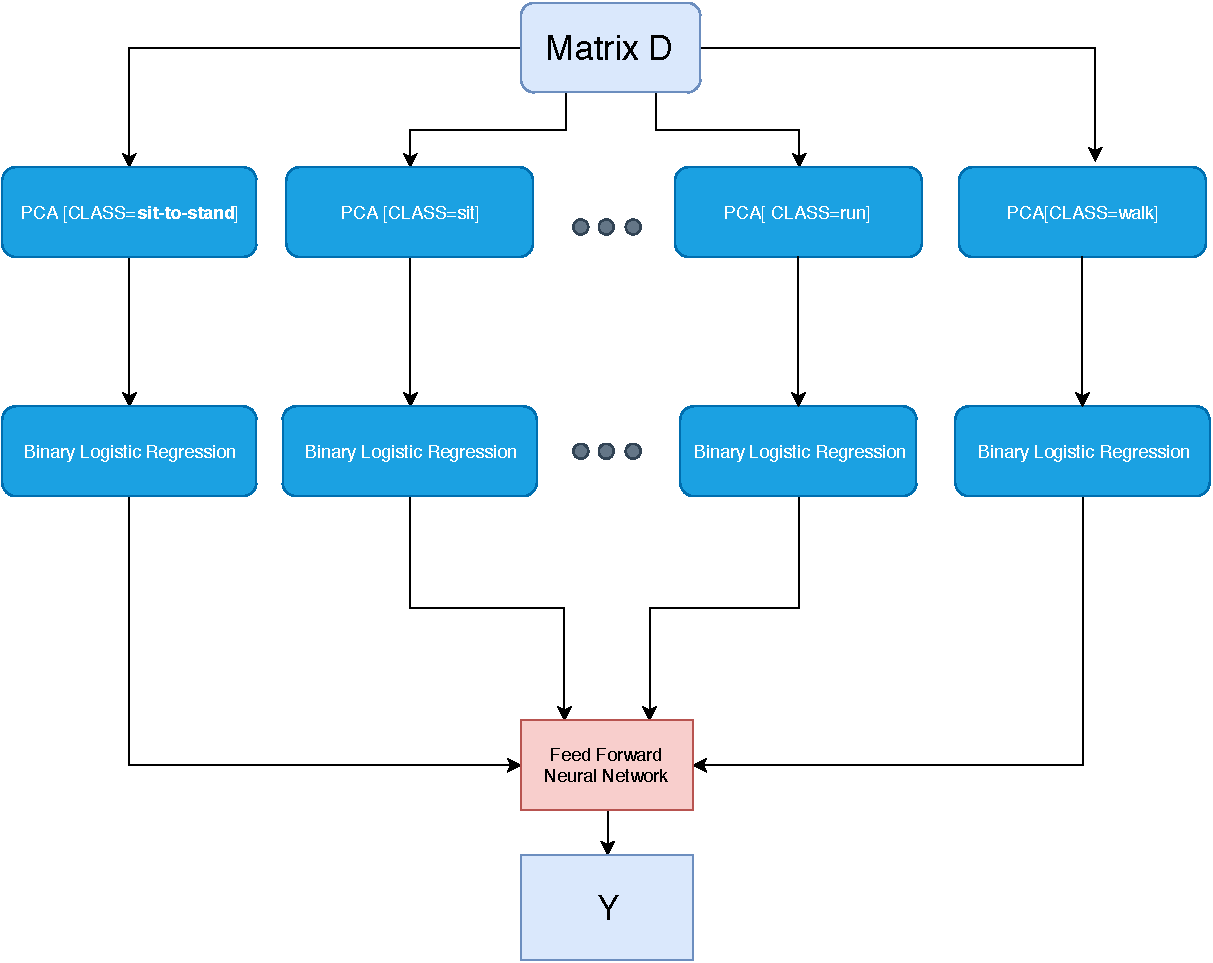
\includegraphics[width=0.7\textwidth]{images/scheme_1.pdf}
	\caption{$\mathcal{P}(\Theta_{1})$  Scheme}
	\label{dig:p1}
\end{figure}

We theorized that the importance of features in matrix $D$ measured by its variance will strongly depend on the particular movement involved, acknowledging this we filtered matrix $D$ by class, and applied principal component analysis $PCA_{|class}: \mathbb{R}^{1079390} \longrightarrow \mathbb{R}^{275}$ to extract the first 275 principal components(this transformation will be the beginning a branch in Figure \ref{dig:p1}) that accounts to 90 $\%$ of the variance. Note that the first level in \ref{dig:p1} has 22 $PCA_{|class}$ extractors. For training, matrix $D$ is passed without filtering per label to each $PCA_{|class}$ and then feed to a \textit{Binary logistic regression} $LogR_{|class}: \mathbb{R}^{275} \longrightarrow [0,1]$ where the classes are encoded in \textit{one vs all} manner. Each of the $LogR_{|class}$ will output a degree of believe that a particular $X$ belows to a class $k$. Finally concatenating the degree of believe predicted by each $LogR_{|class}$ we construct a $X' \in \mathbb{R}^{22}$. Finally $X'$ is passed to a single feed forward neuronal network $NN: \mathbb{R}^{22} \longrightarrow  \mathbb{R}^{22} $ that predicts our final probability vector $Y$ in a \textit{hot encoded} structure, we take the maximum component and assign its corresponding label to that register.


\begin{equation}
\Theta_{1}:= \{ Preprocessing_{ \ method \ 1},PCA_{|class},LogR_{|class},NN \}
\label{eq:1}
\end{equation}


\subsection{Data Exploitation with $Preprocessing_{ \ method \ 2}$}
The dimension of $X$ using $Preprocessing_{ \ method \ 2}$ is $R^{152}$ so no further dimension reduction is required. We implemented a variety of feed forward neuron networks using tensor flow, where we varied the Network architecture composed by the number of hidden units $H_{units} \in \mathbb{N}^{>0}$ per hidden layer $H_{L} \in \mathbb{N}^{>0}$ the regularization parameter $\alpha \in \mathbb{R}^{>0}$, and the activation functions, namely $ \{  Logistic, tanh, relu \}$. From Figures \ref{sm1} to  \ref{sm22} we can observe $\mu$ signal examples per label.

\begin{equation}
\Theta_{2}:= \{ Preprocessing_{ \ method \ 2},NN \}
\label{eq:2}
\end{equation}


\begin{figure}[!tbp]
	\begin{minipage}[b]{0.31\textwidth}
		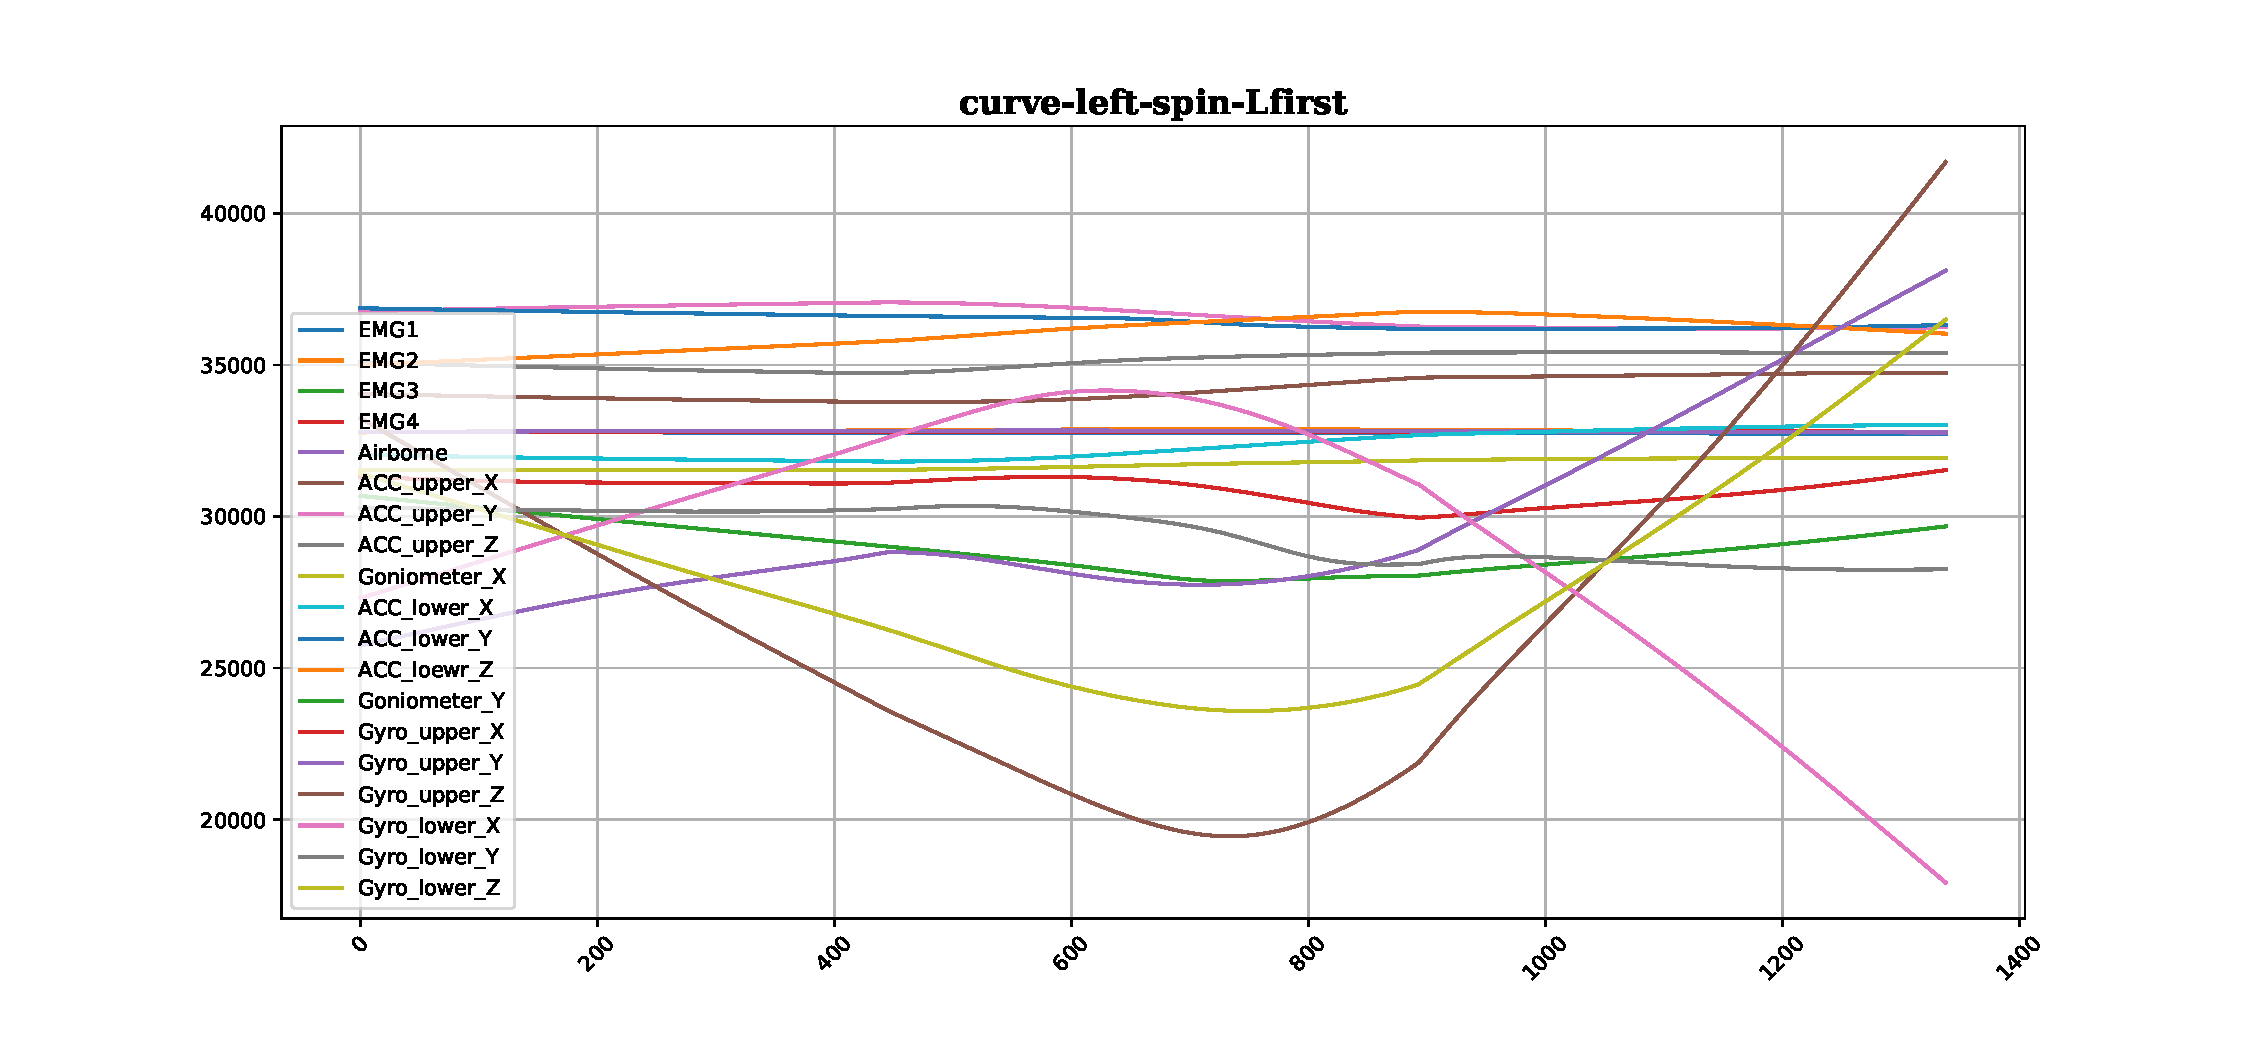
\includegraphics[width=\textwidth]{images/curve-left-spin-Lfirst_example.pdf}
		\caption{curve-left-spin-Lfirst}
		\label{sm1}
	\end{minipage}
	\begin{minipage}[b]{0.31\textwidth}
		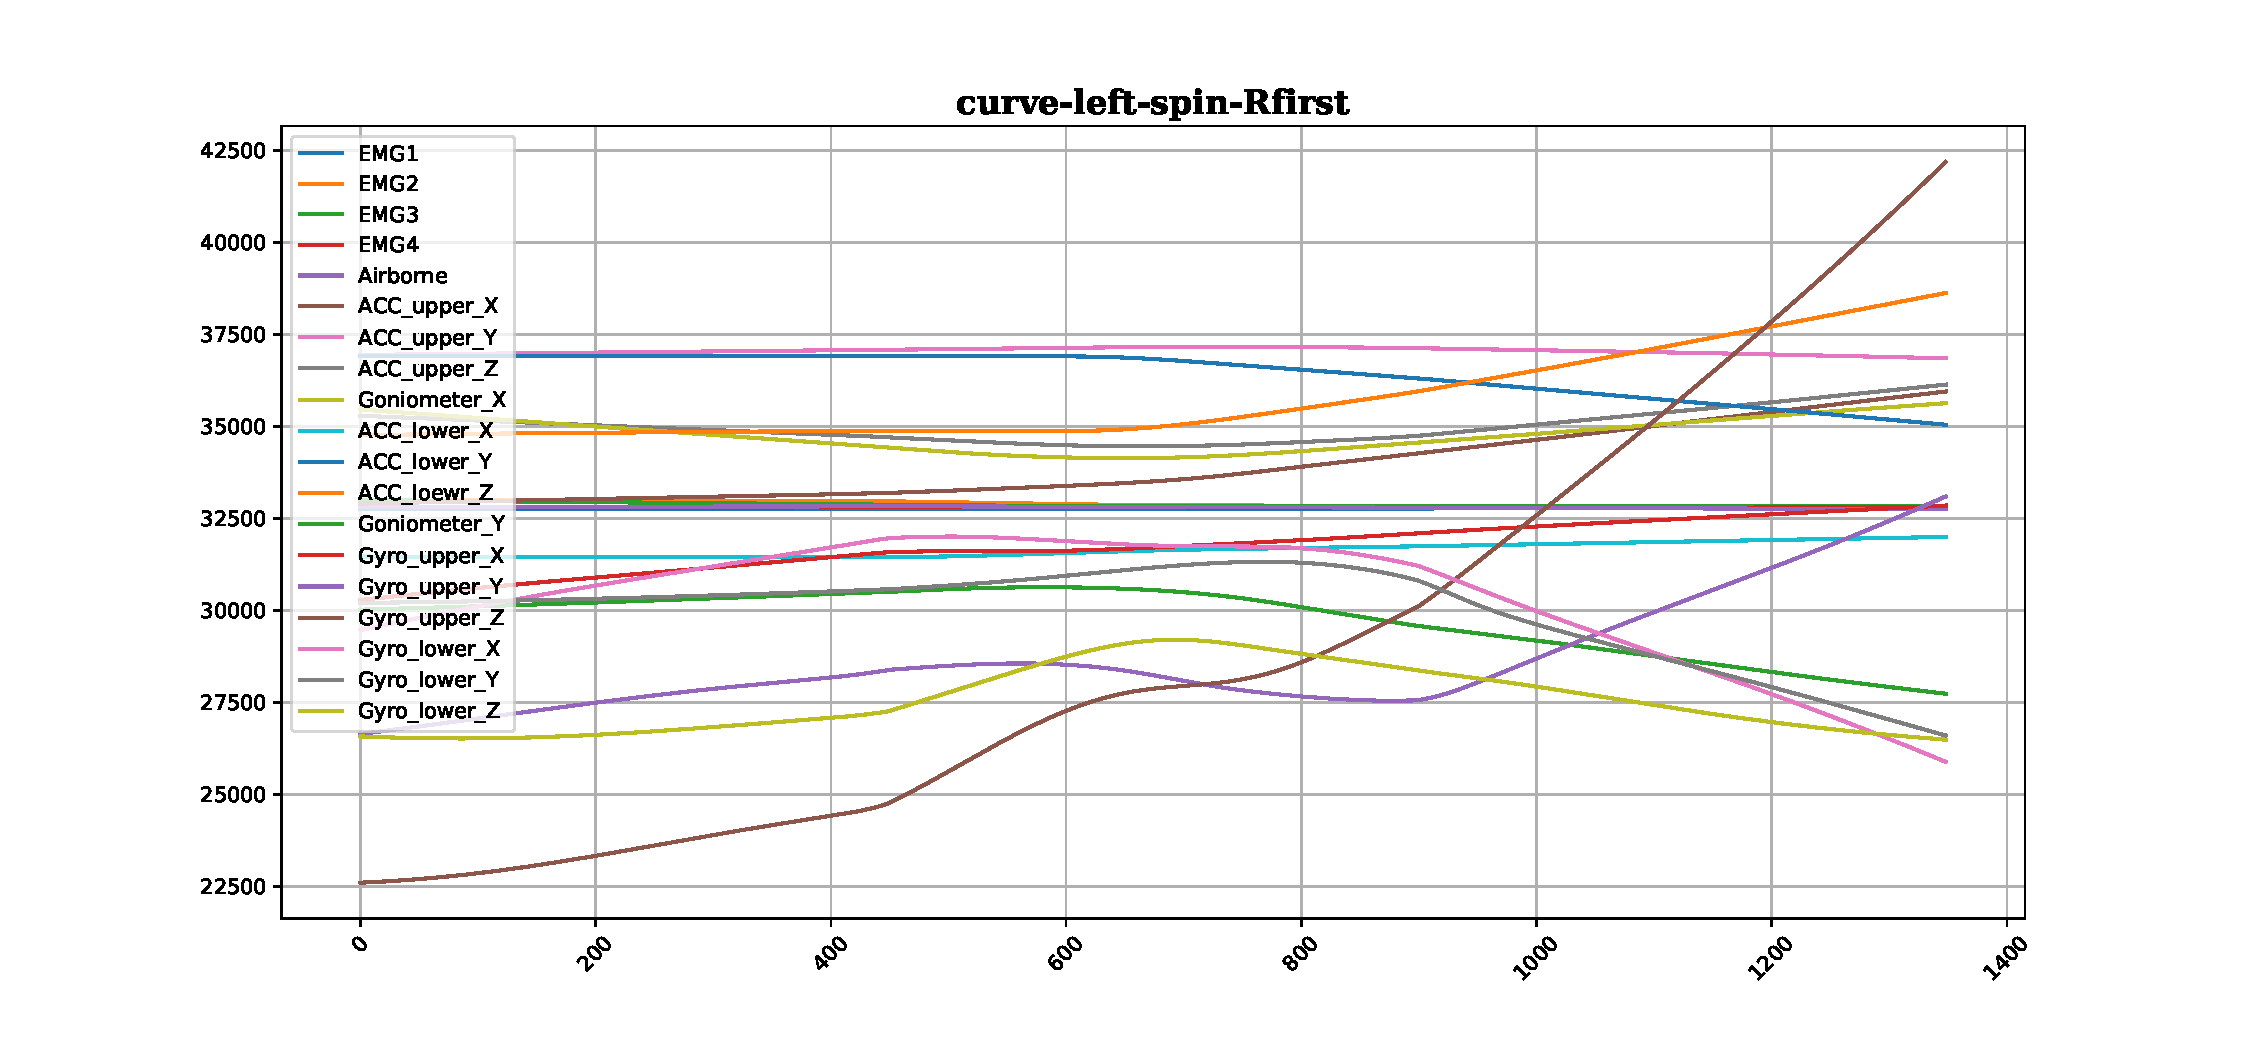
\includegraphics[width=\textwidth]{images/curve-left-spin-Rfirst_example.pdf}
		\caption{curve-left-spin-Rfirst}
	\end{minipage}
	\begin{minipage}[b]{0.31\textwidth}
		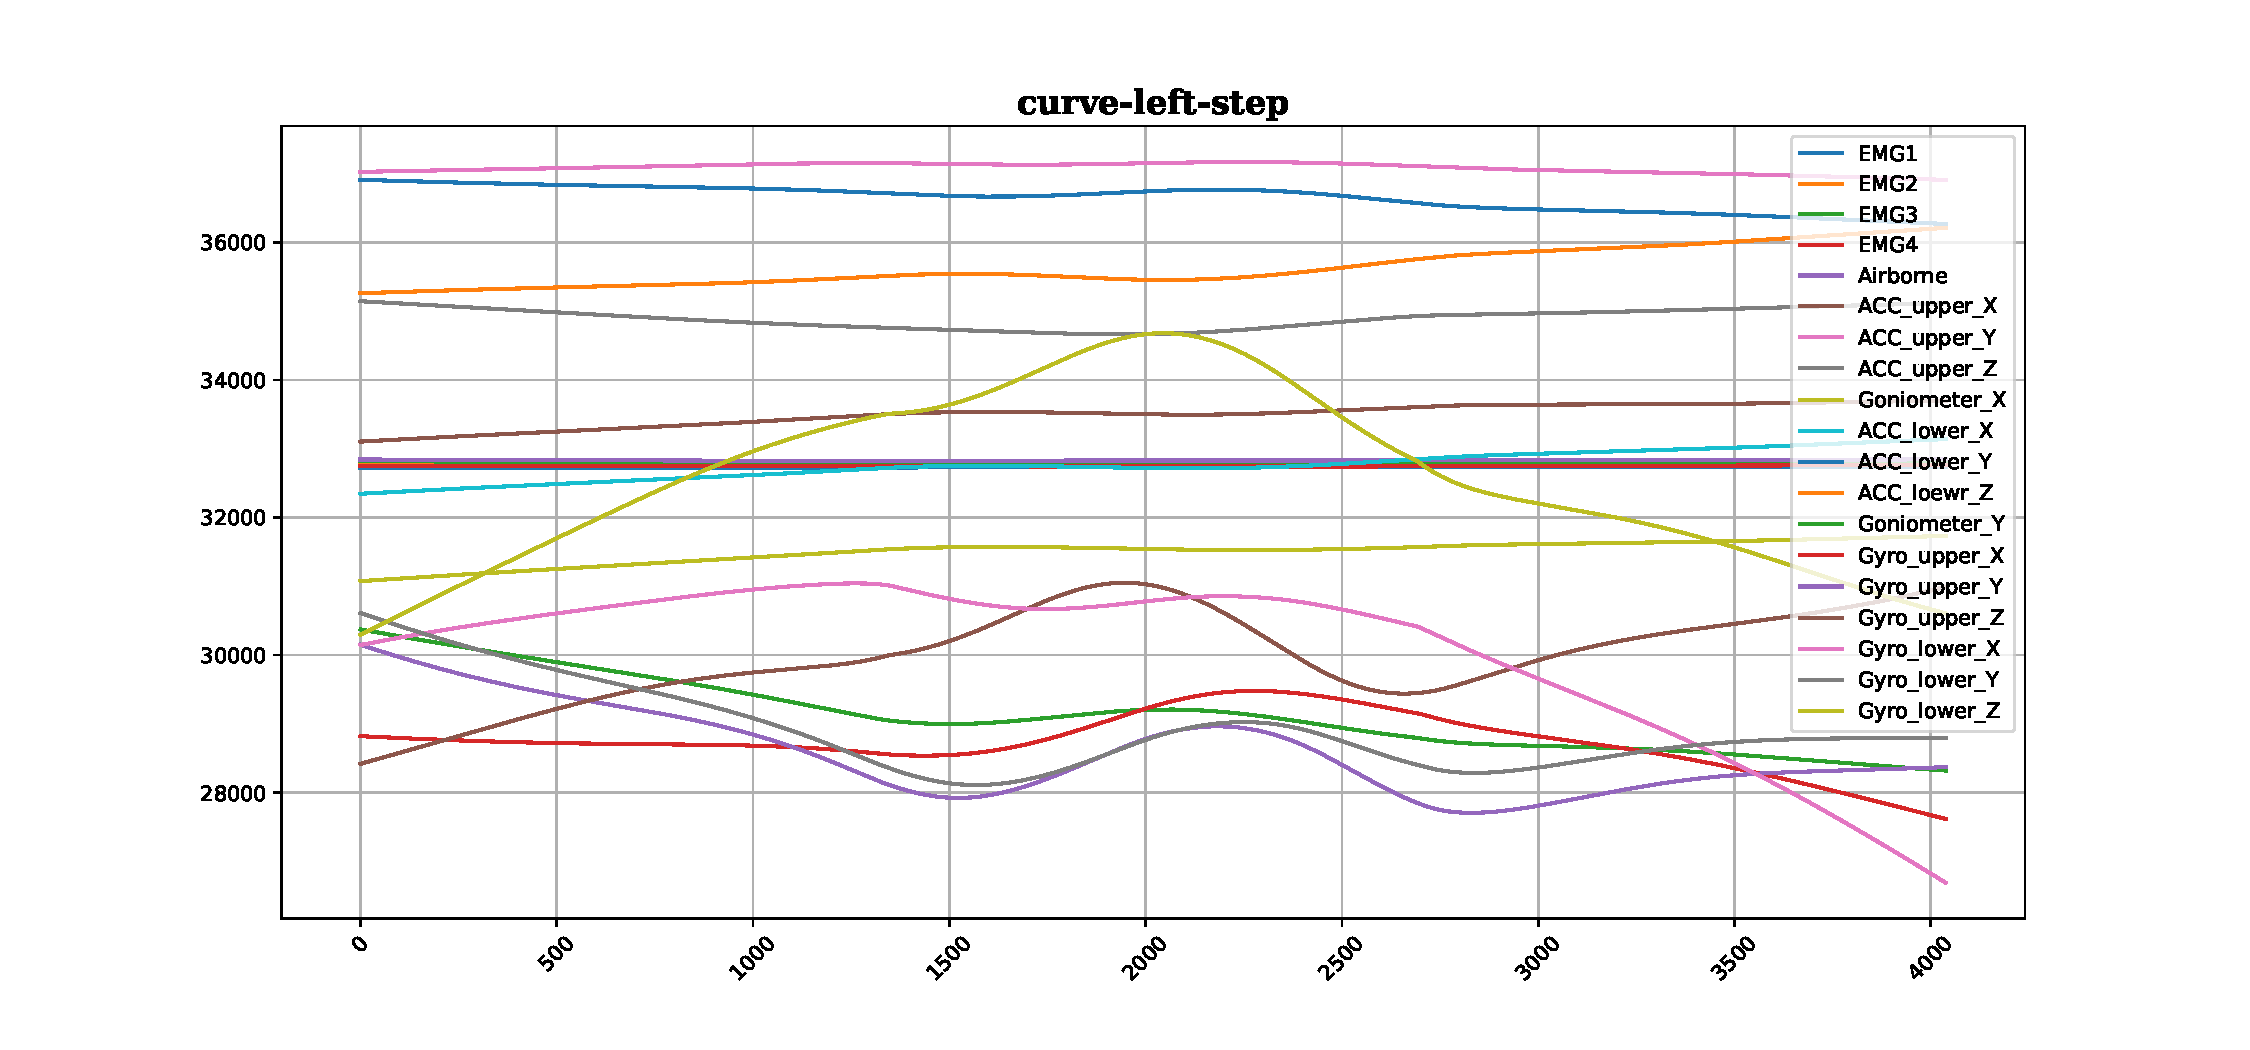
\includegraphics[width=\textwidth]{images/curve-left-step_example.pdf}
		\caption{curve-left-step}
	\end{minipage}
\end{figure}

\begin{figure}[!tbp]
	\begin{minipage}[b]{0.31\textwidth}
		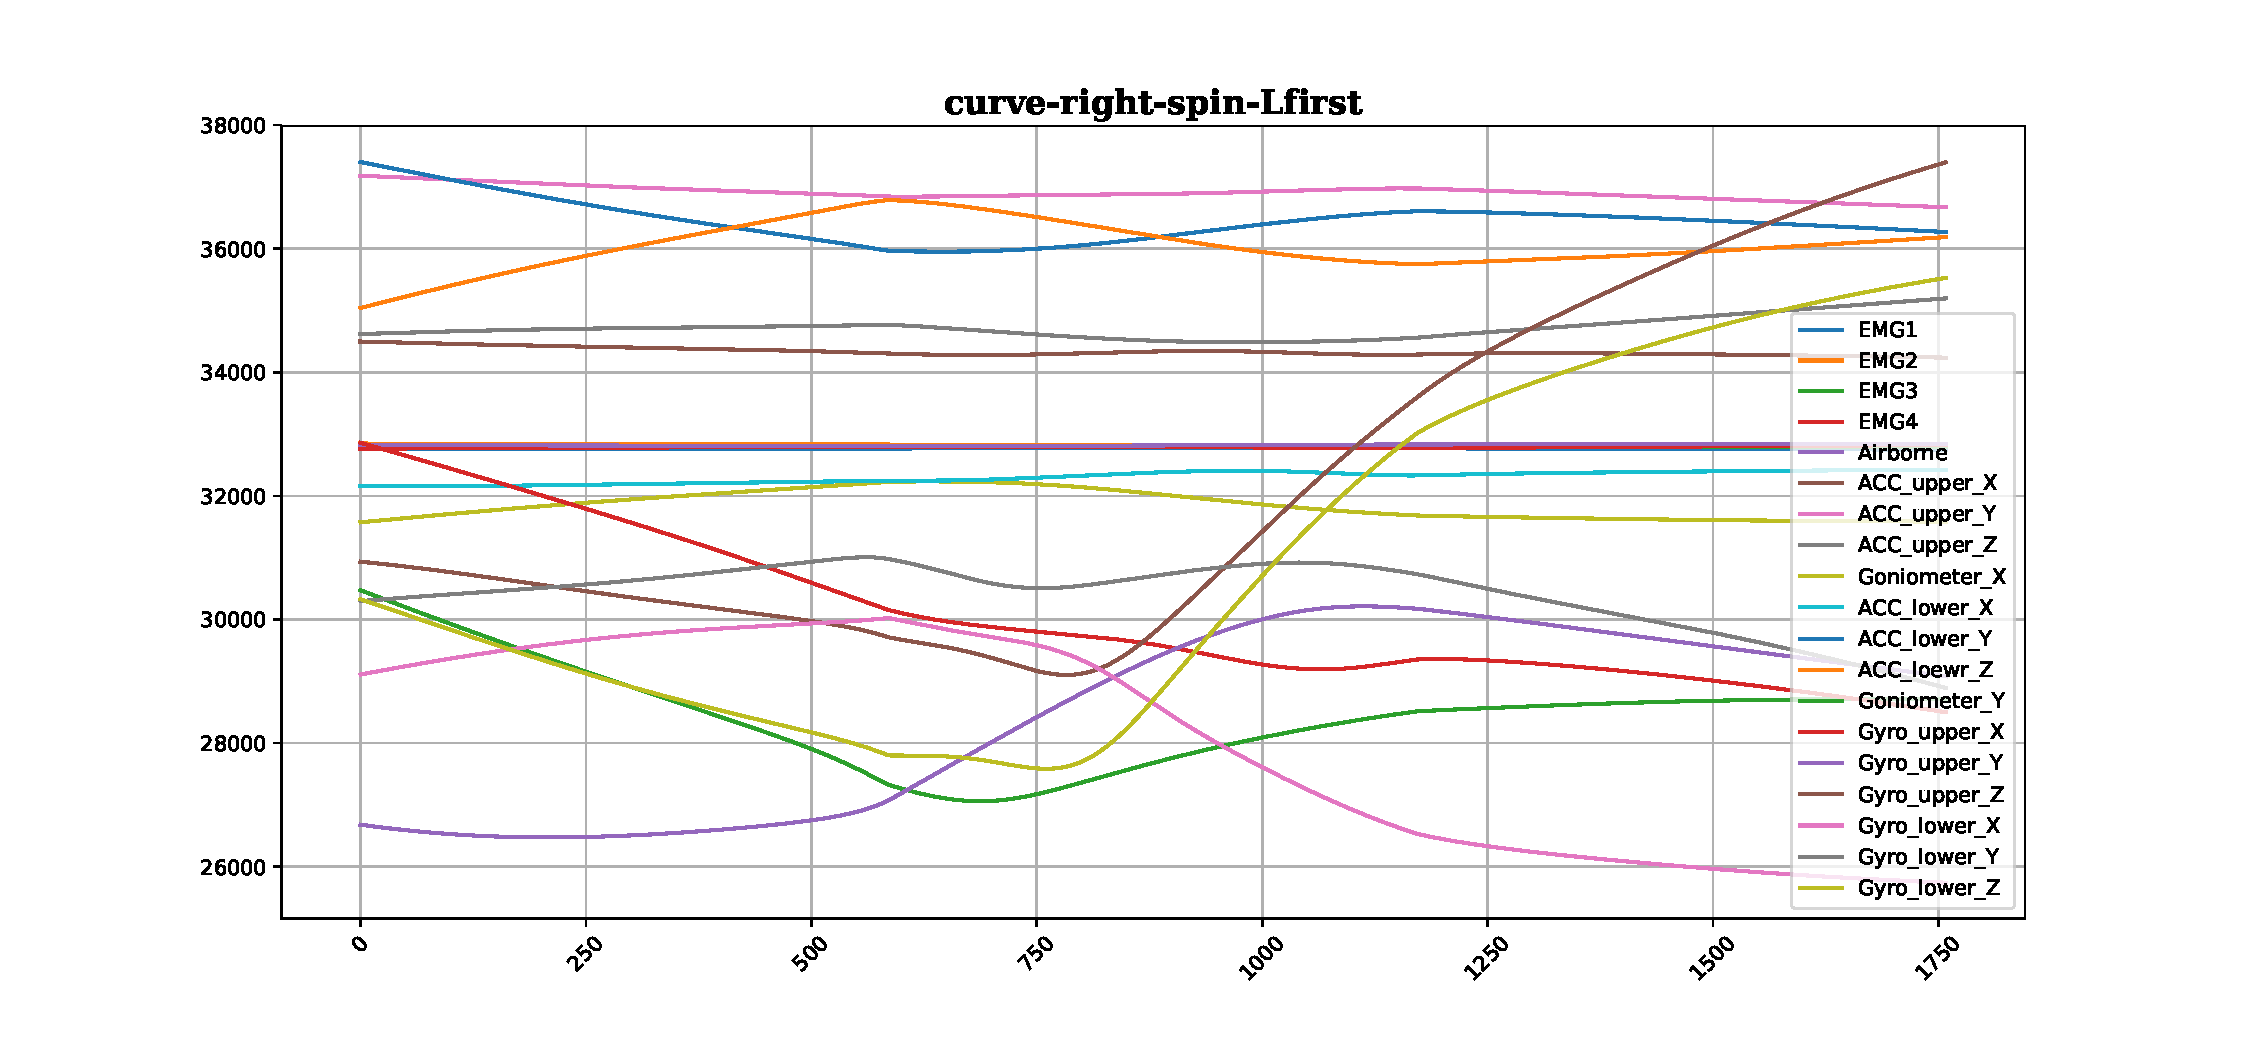
\includegraphics[width=\textwidth]{images/curve-right-spin-Lfirst_example.pdf}
		\caption{curRight-spin-Lfirst}
	\end{minipage}
	\begin{minipage}[b]{0.31\textwidth}
		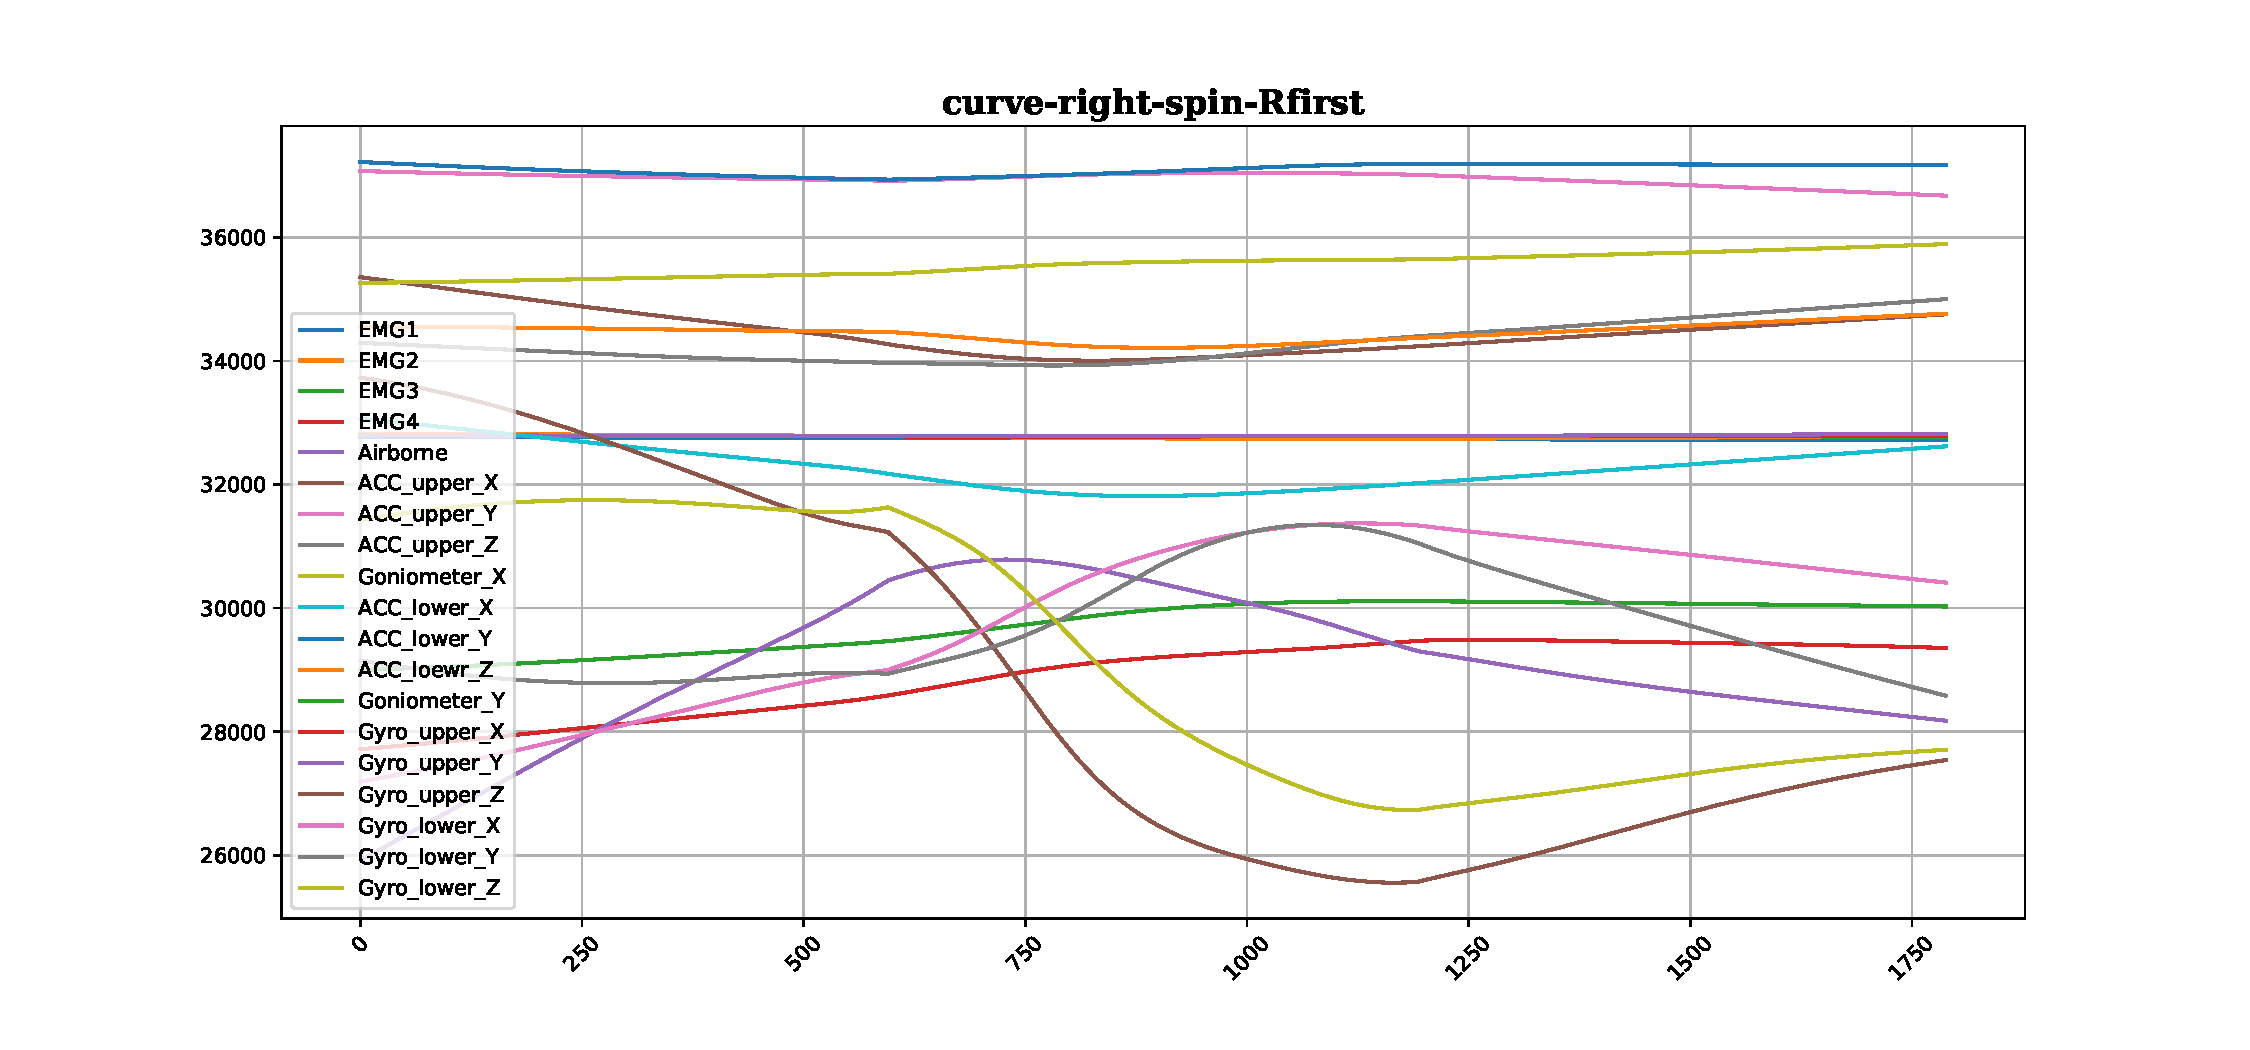
\includegraphics[width=\textwidth]{images/curve-right-spin-Rfirst_example.pdf}
		\caption{curRight-spin-Rfirst}
	\end{minipage}
	\begin{minipage}[b]{0.31\textwidth}
		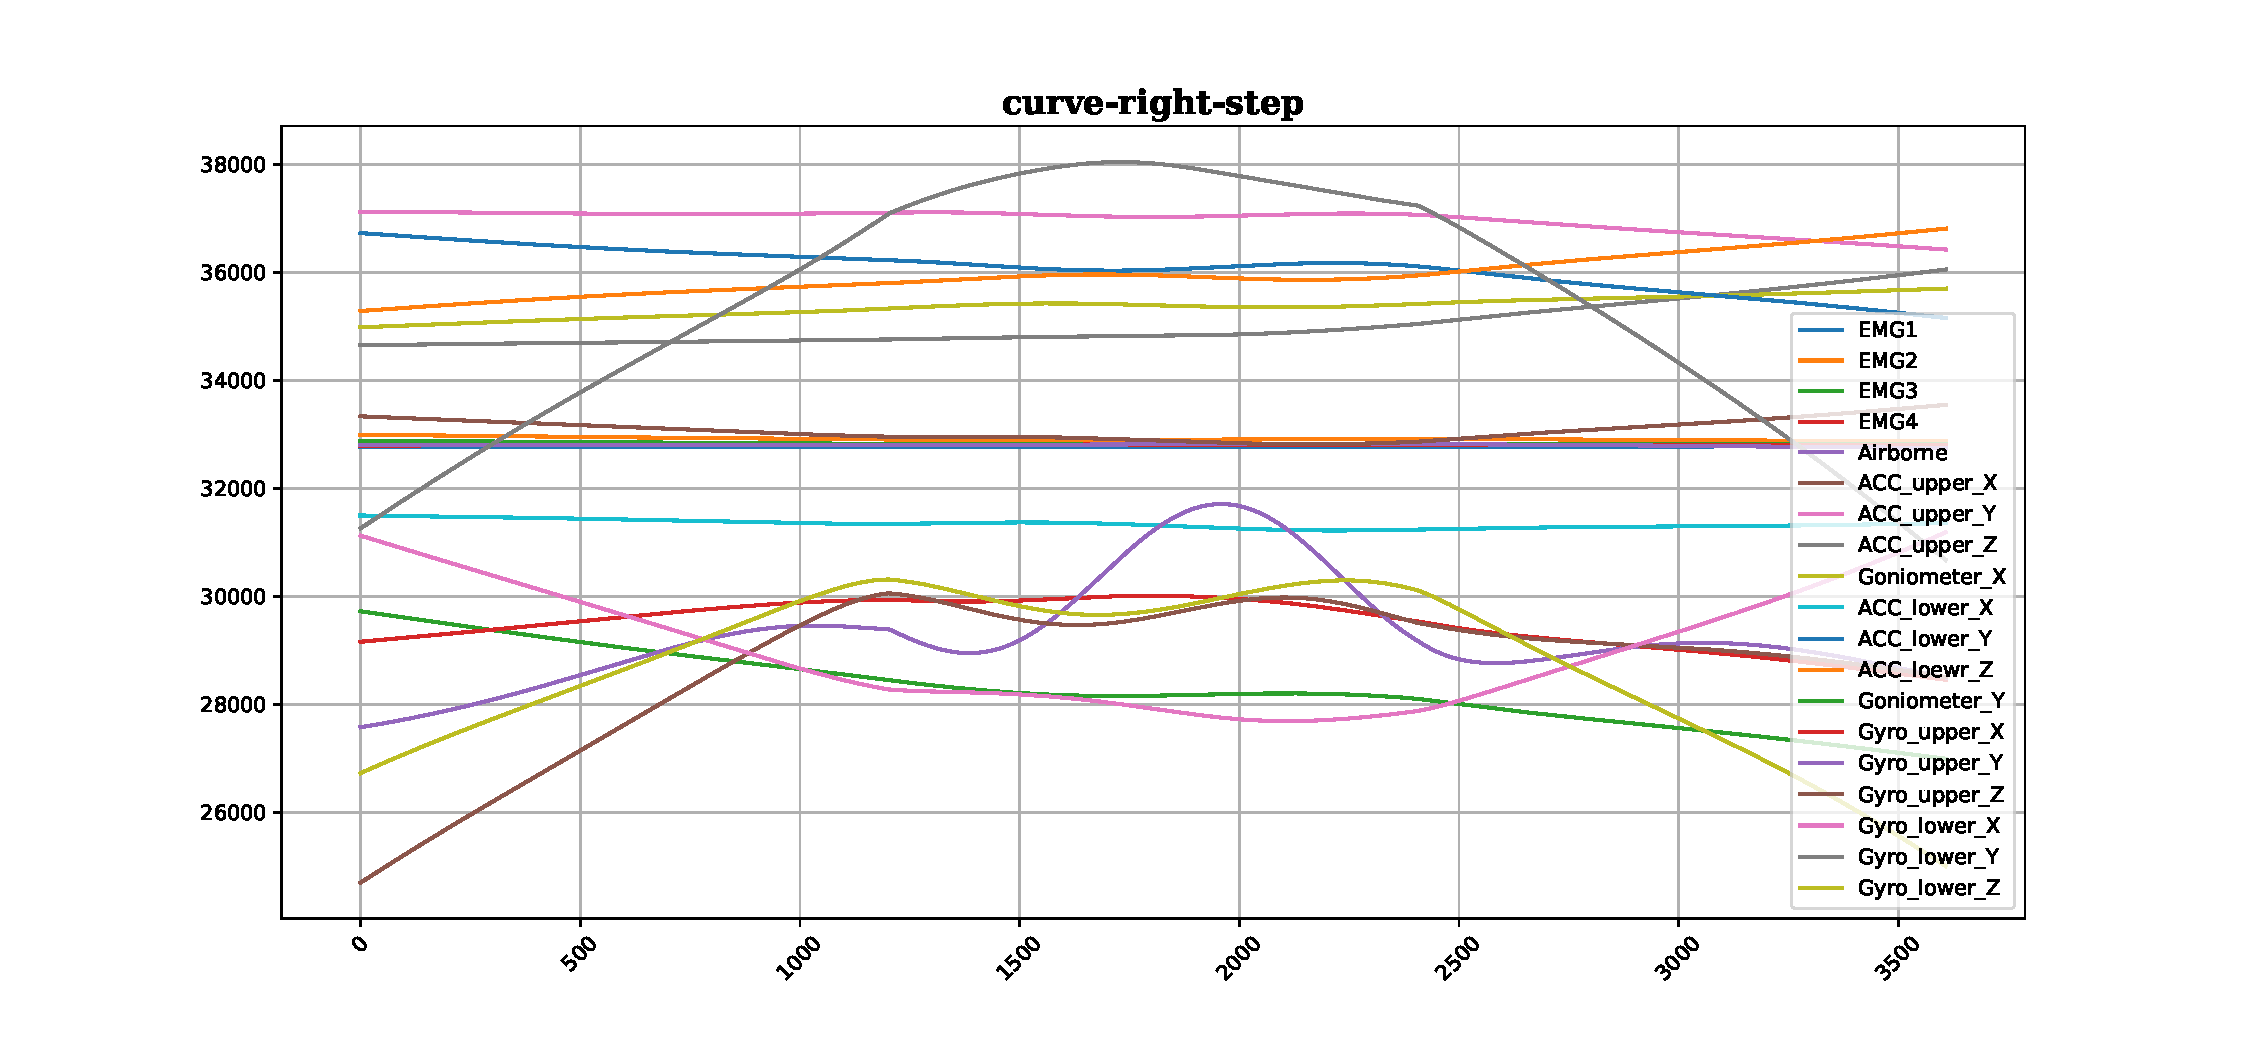
\includegraphics[width=\textwidth]{images/curve-right-step_example.pdf}
		\caption{curRight-step}
	\end{minipage}
\end{figure}



\begin{figure}[!tbp]
	\begin{minipage}[b]{0.31\textwidth}
		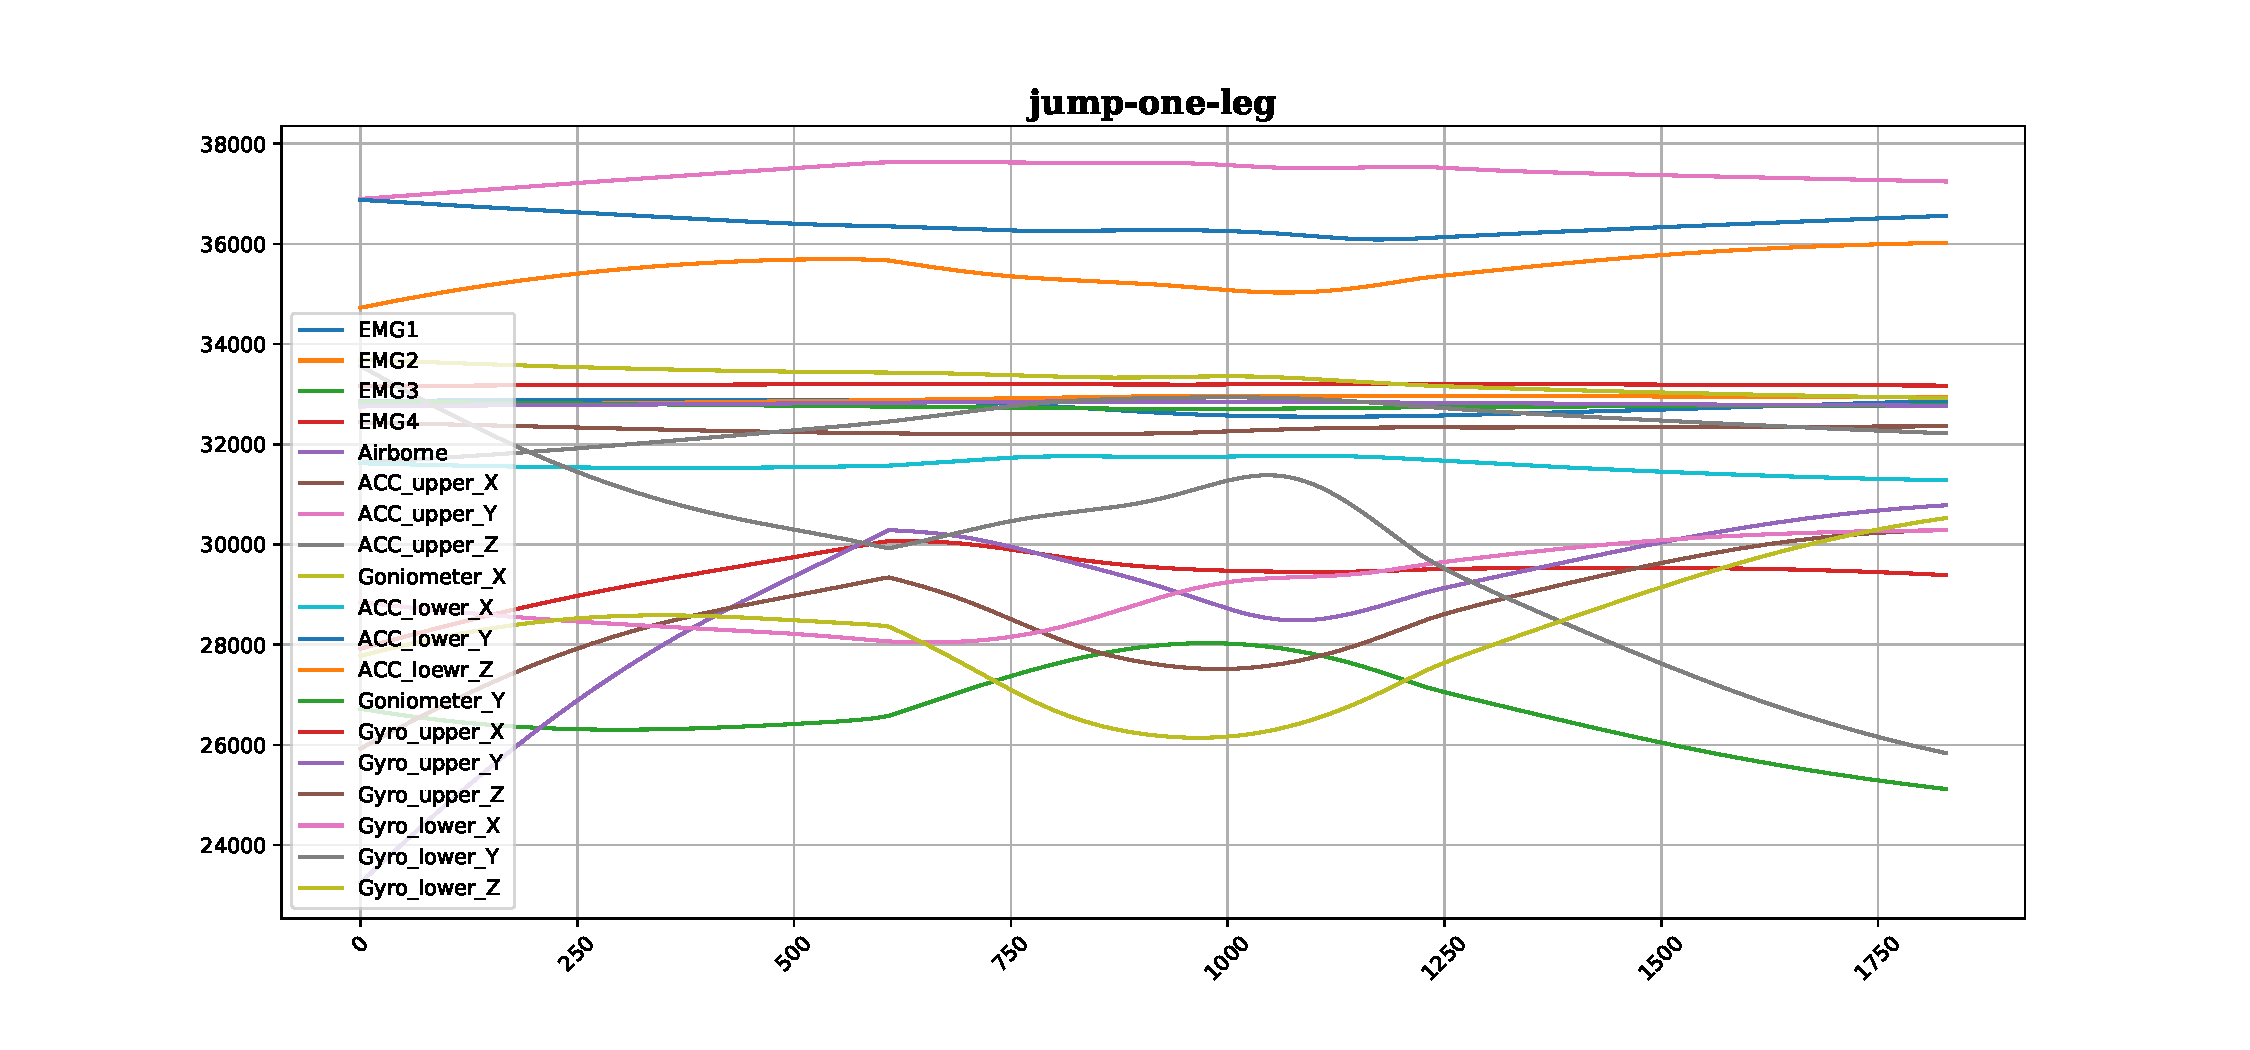
\includegraphics[width=\textwidth]{images/jump-one-leg_example.pdf}
		\caption{jump-one-leg}
	\end{minipage}
	\begin{minipage}[b]{0.31\textwidth}
		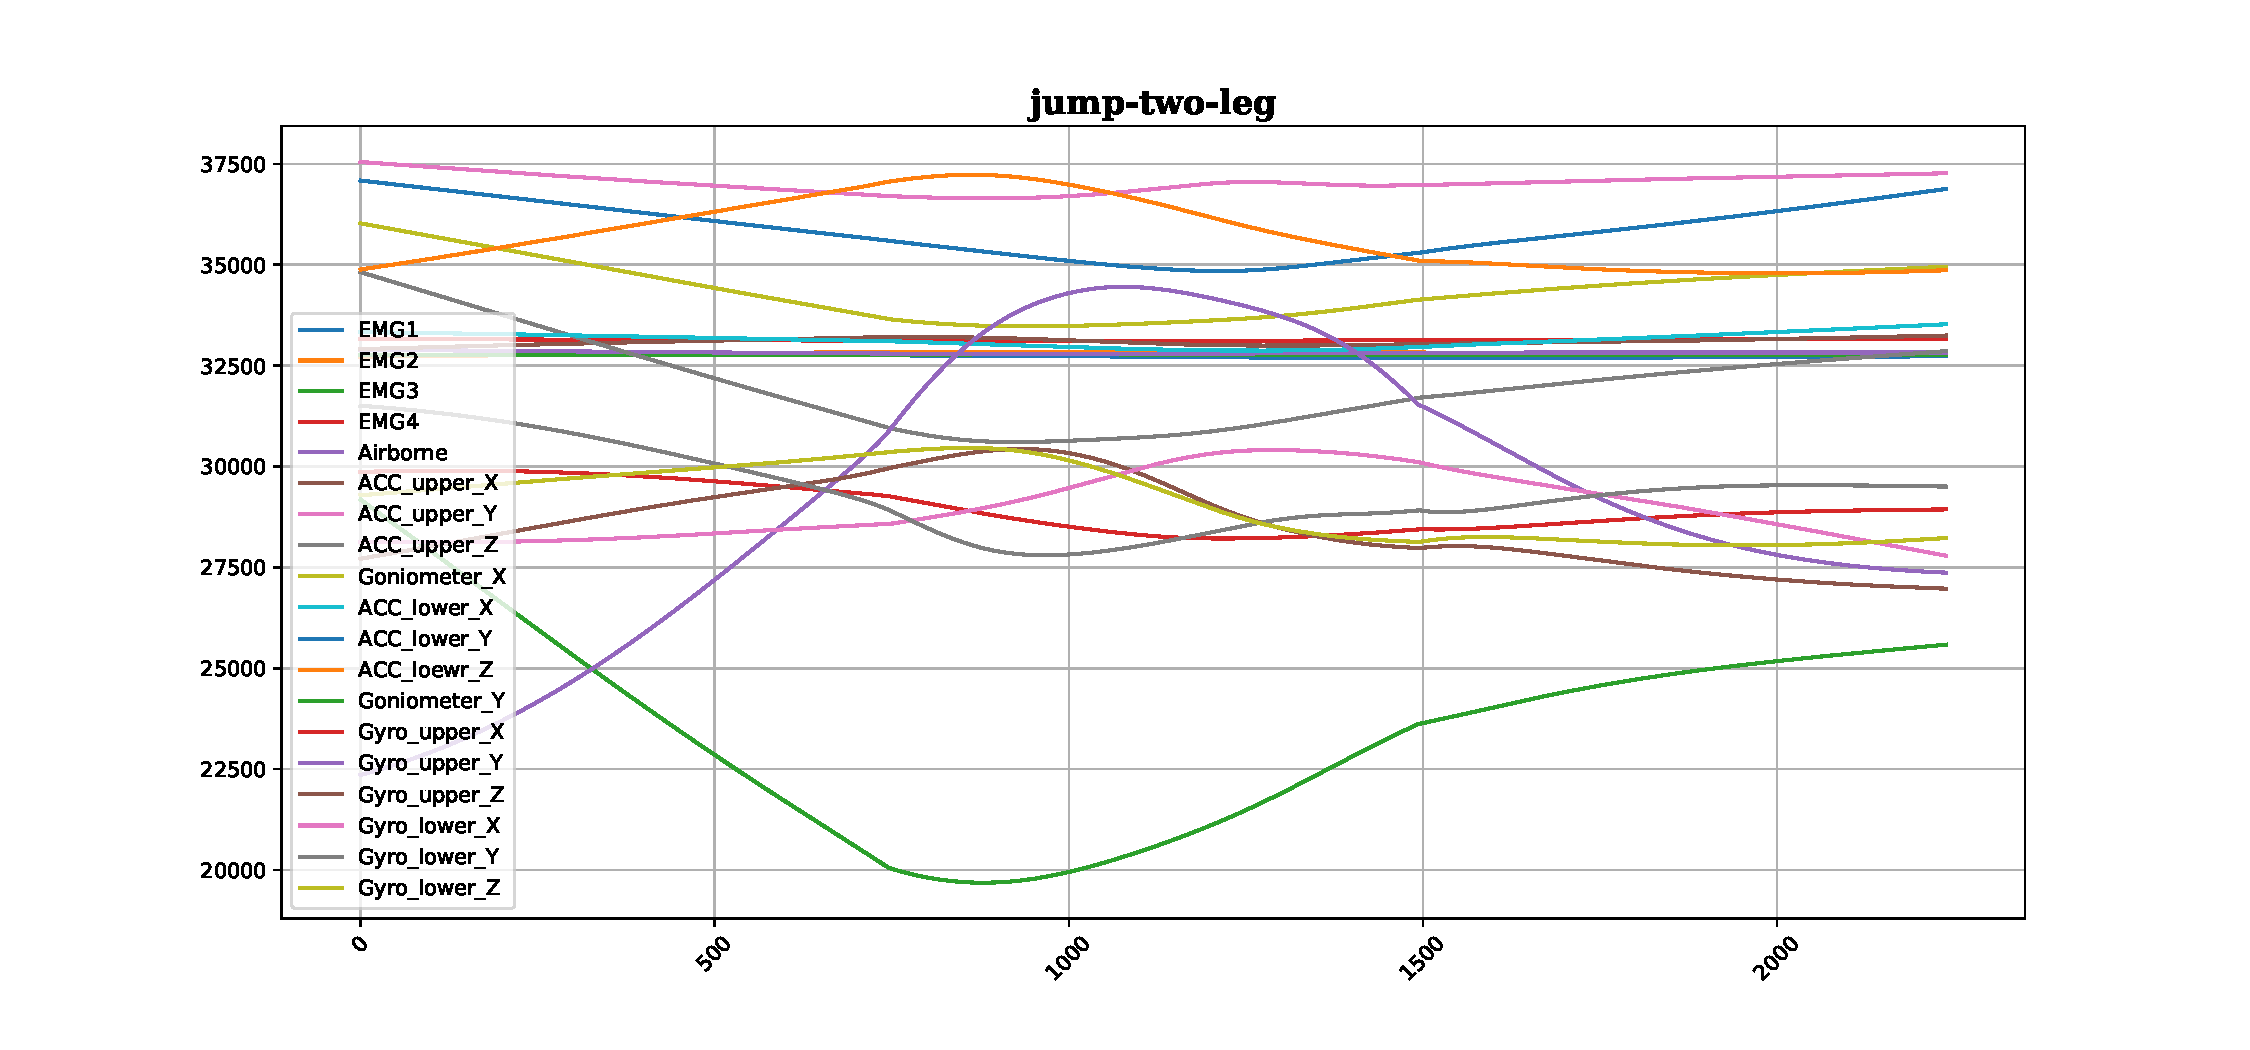
\includegraphics[width=\textwidth]{images/jump-two-leg_example.pdf}
		\caption{jump-two-leg}
	\end{minipage}
	\begin{minipage}[b]{0.31\textwidth}
		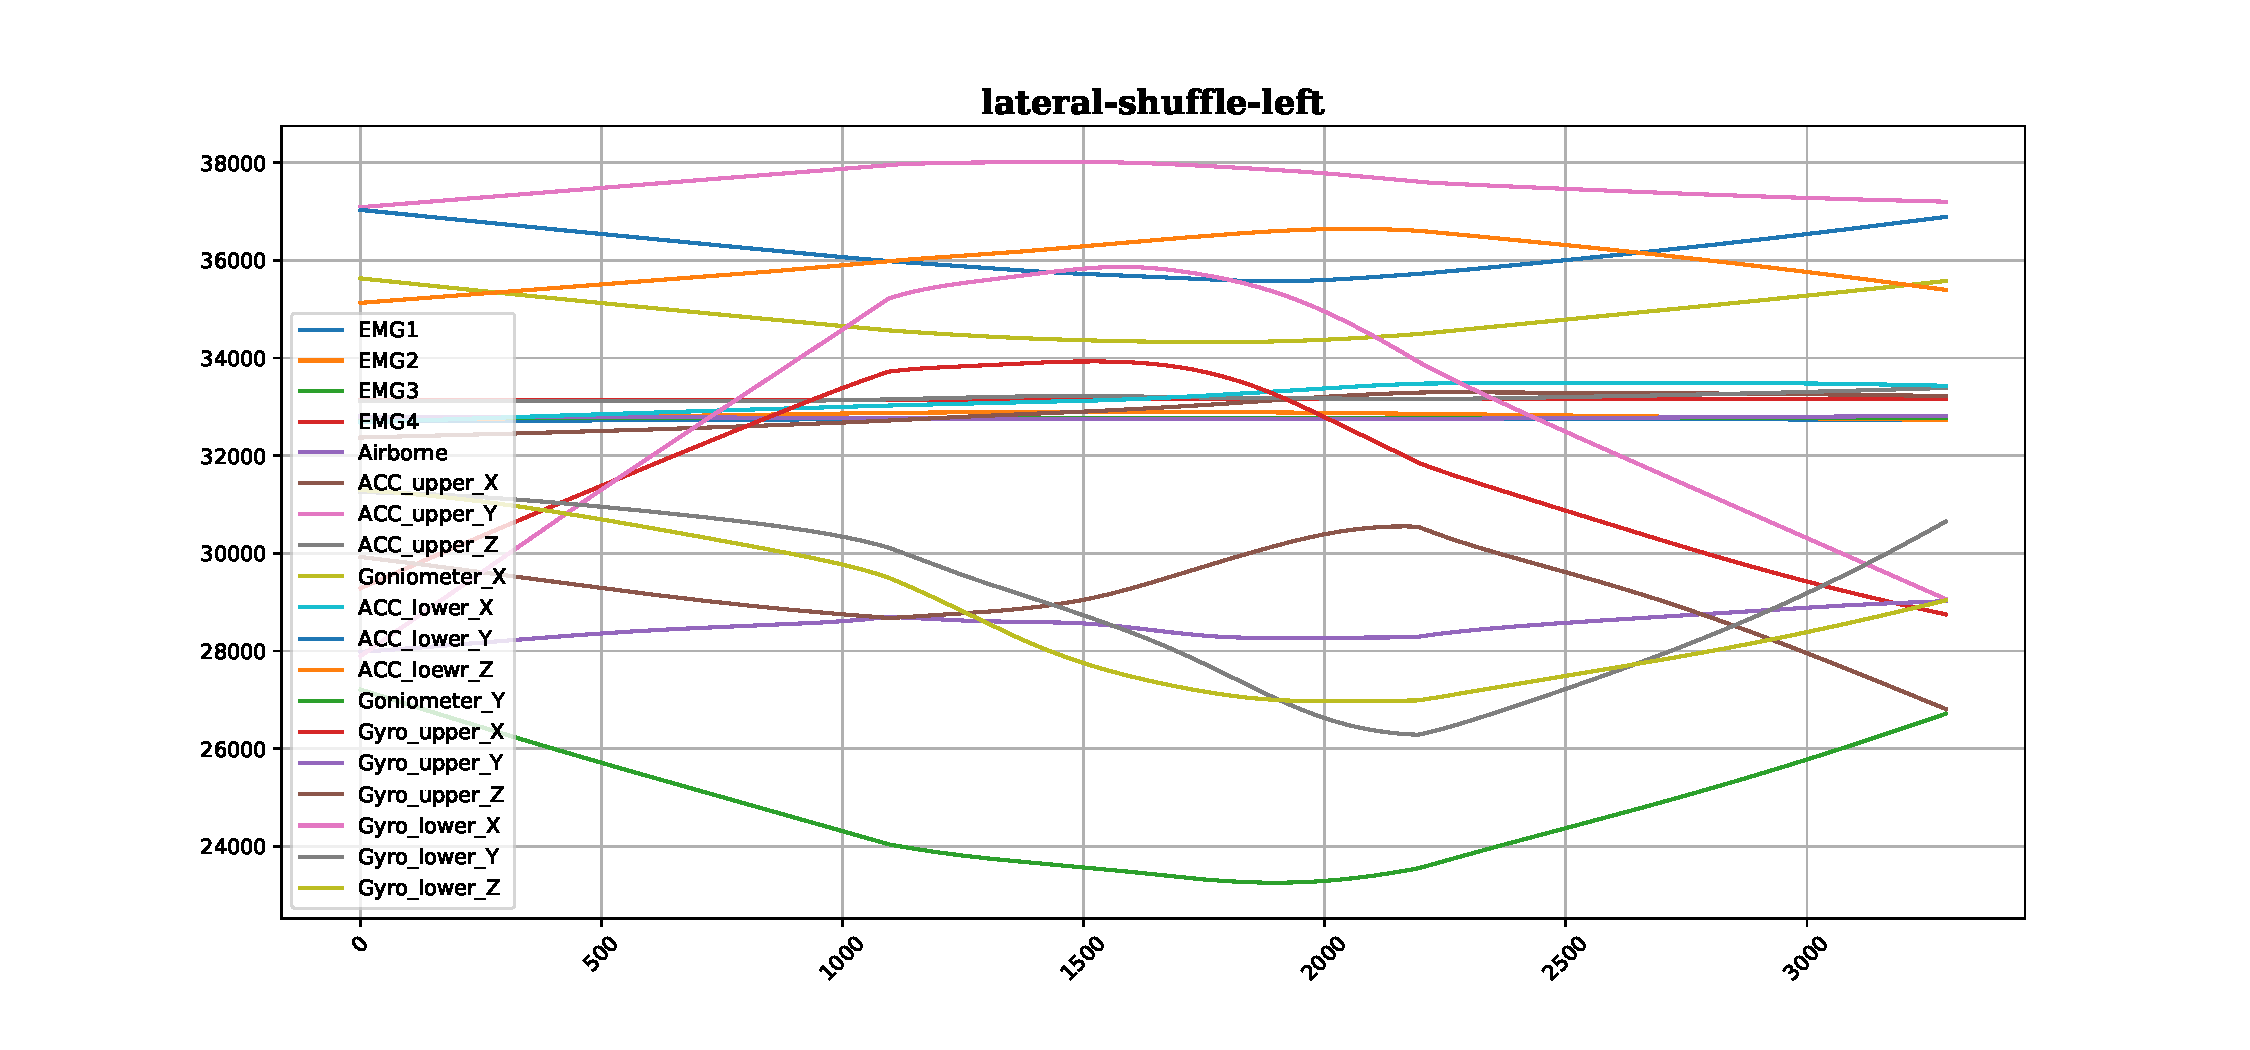
\includegraphics[width=\textwidth]{images/lateral-shuffle-left_example.pdf}
		\caption{lateral-shuffle-left}
	\end{minipage}
\end{figure}


\begin{figure}[!tbp]
	\begin{minipage}[b]{0.31\textwidth}
		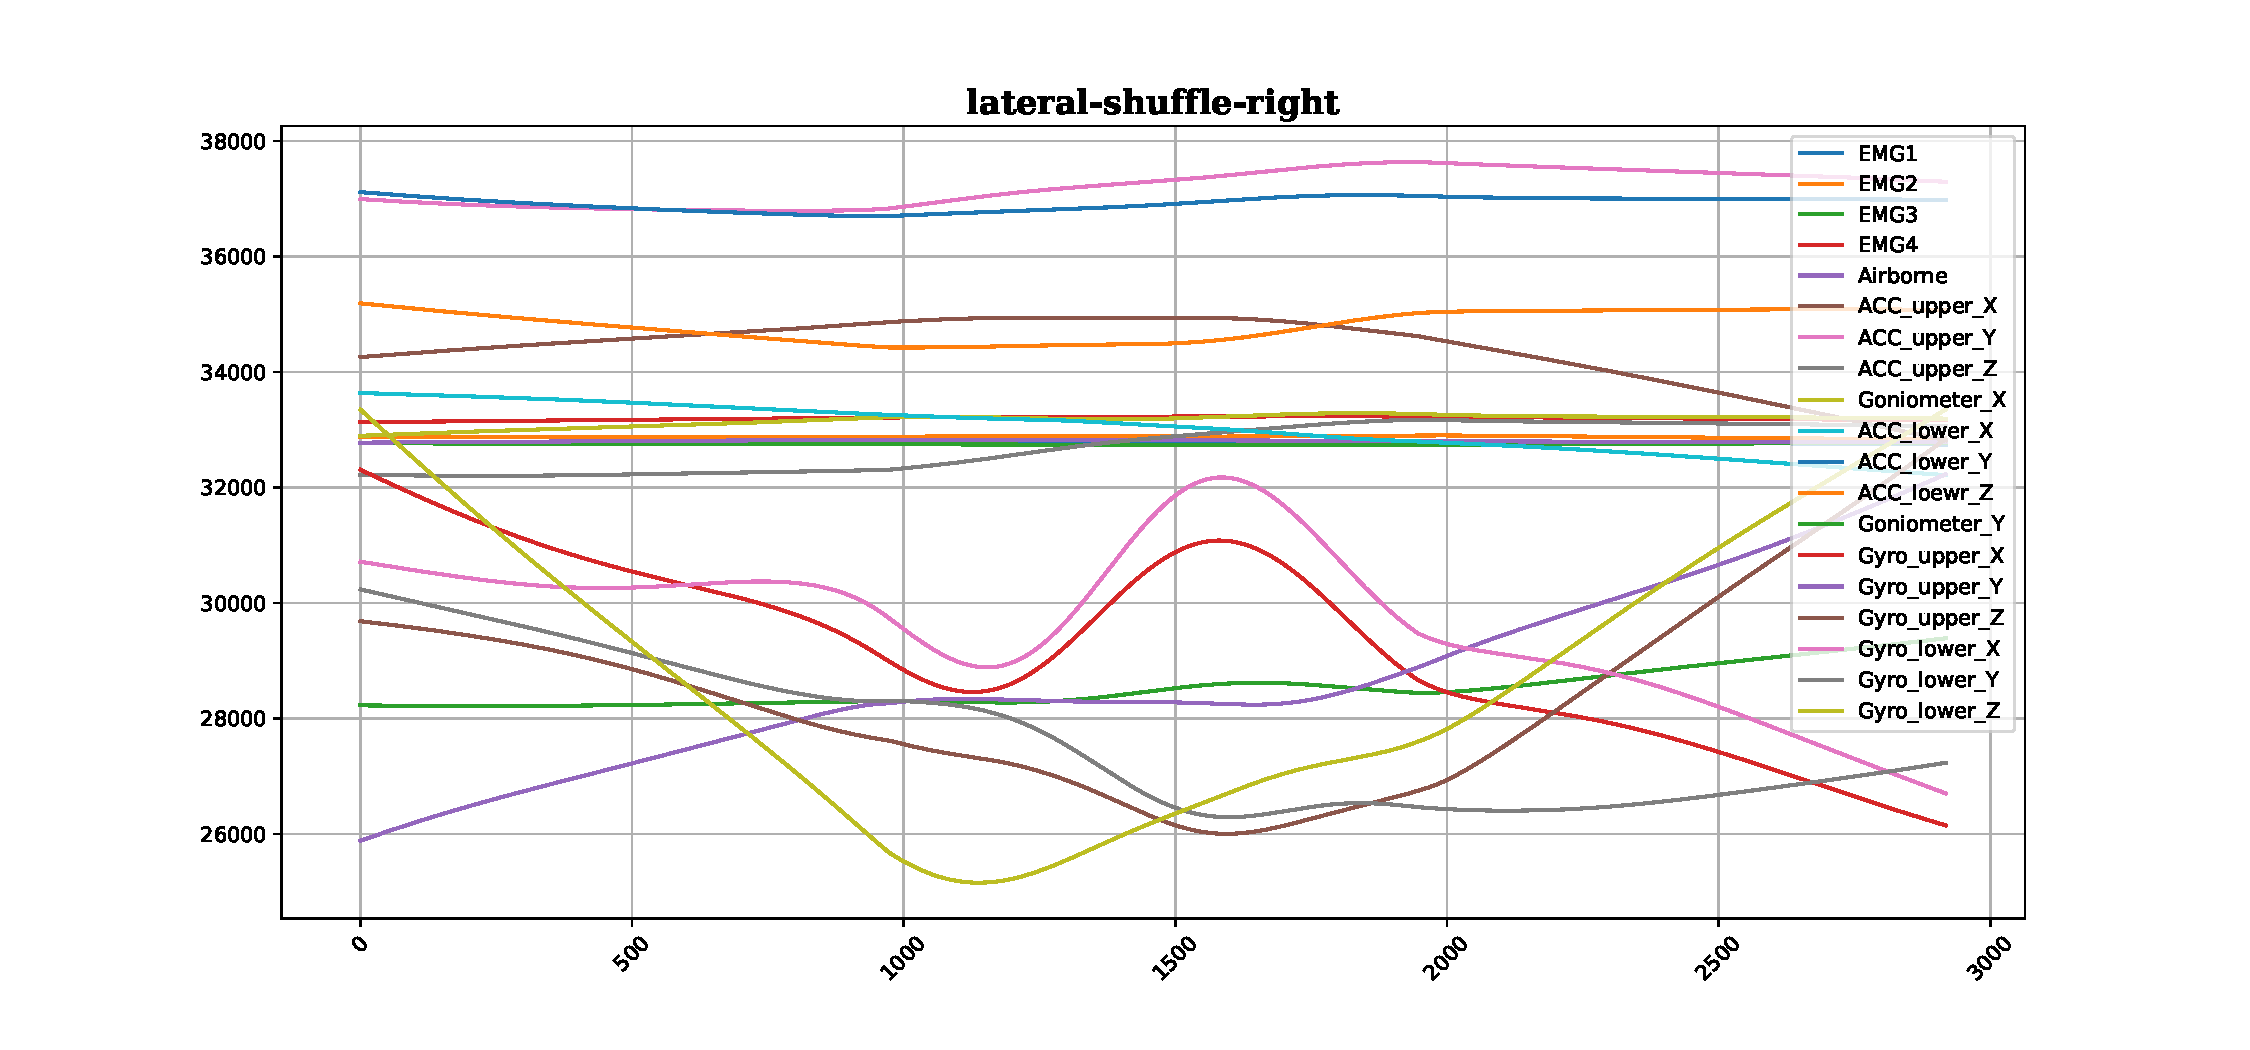
\includegraphics[width=\textwidth]{images/lateral-shuffle-right_example.pdf}
		\caption{lateral-shuffle-right}
	\end{minipage}
	\begin{minipage}[b]{0.31\textwidth}
		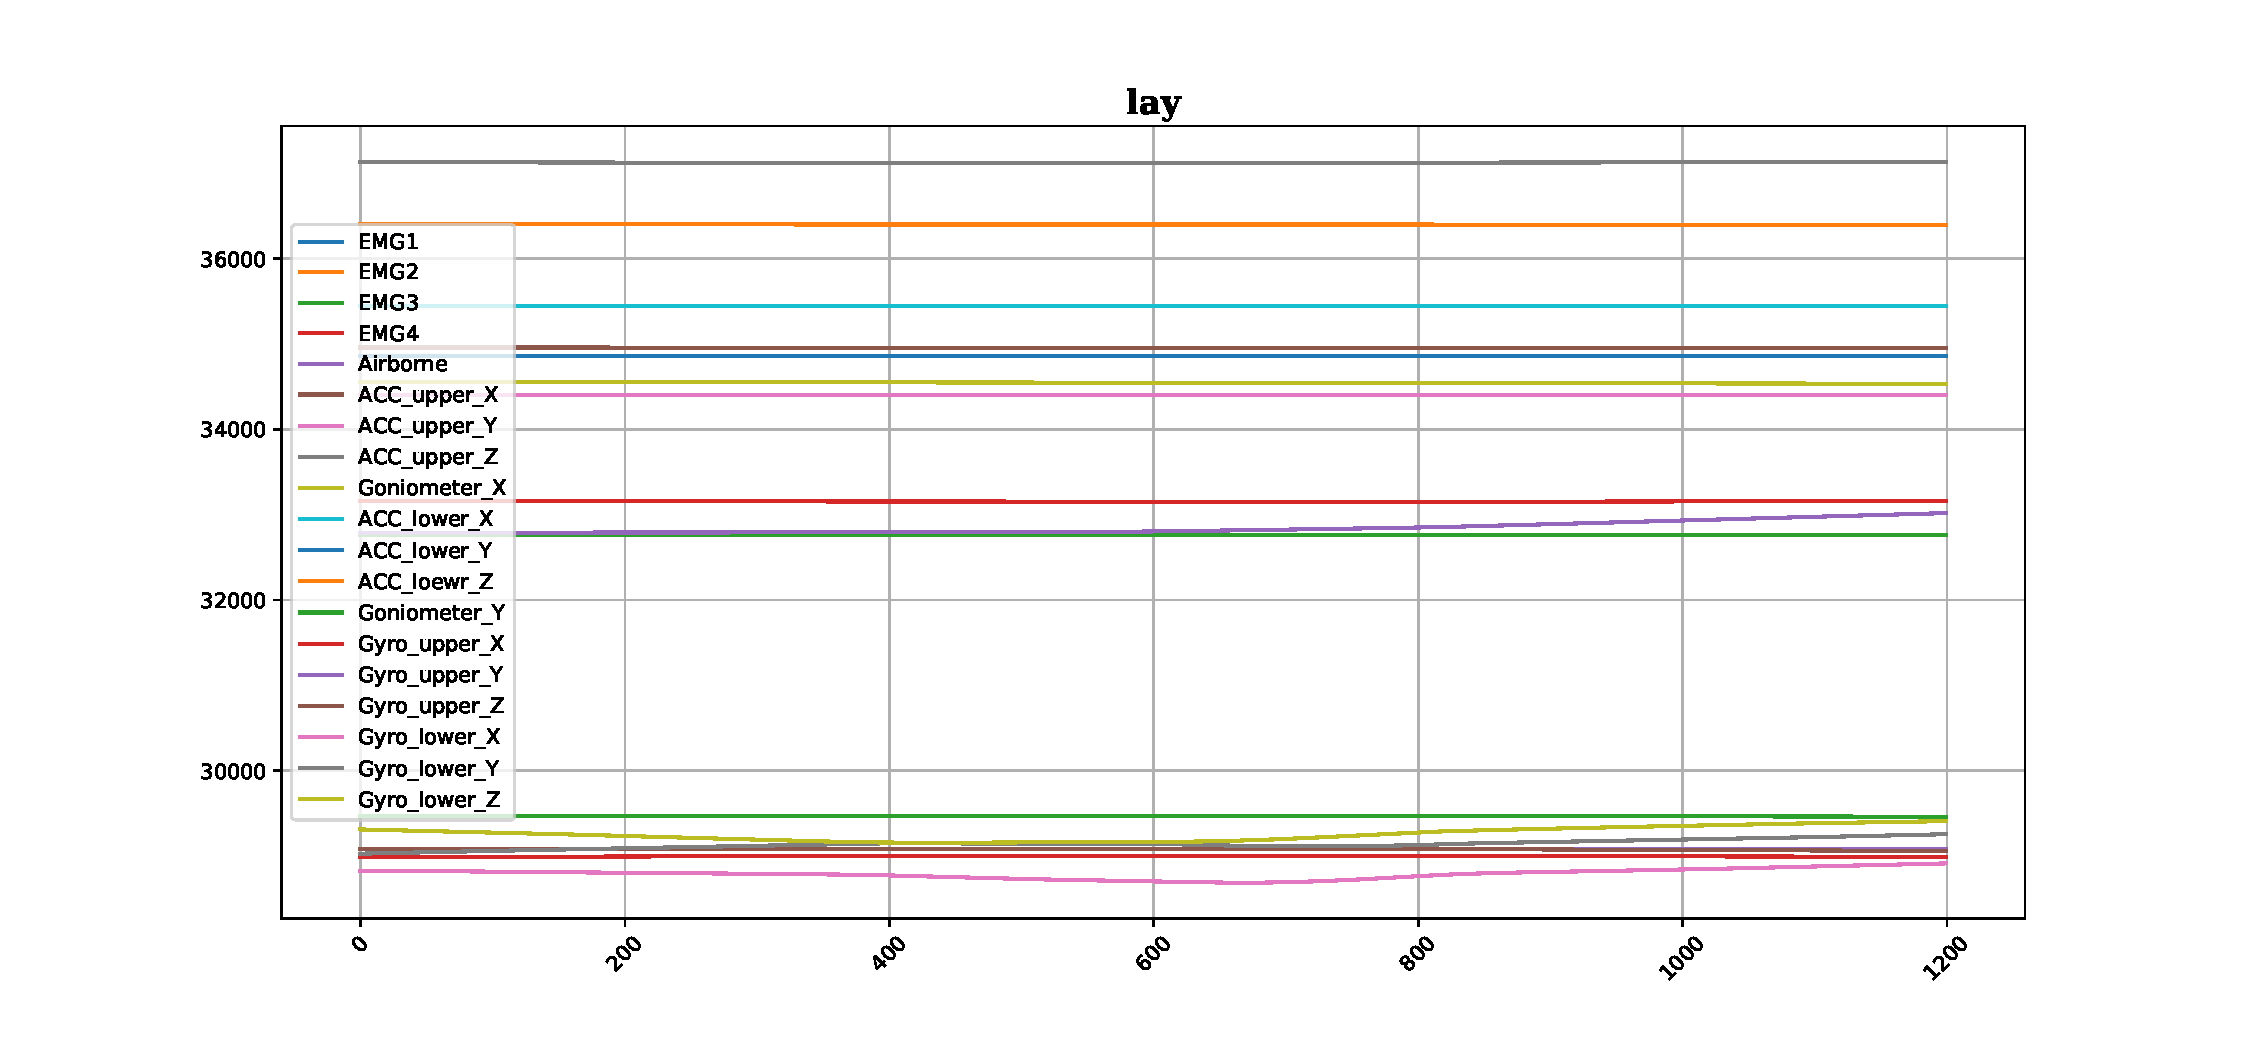
\includegraphics[width=\textwidth]{images/lay_example.pdf}
		\caption{lay}
	\end{minipage}
	\begin{minipage}[b]{0.31\textwidth}
		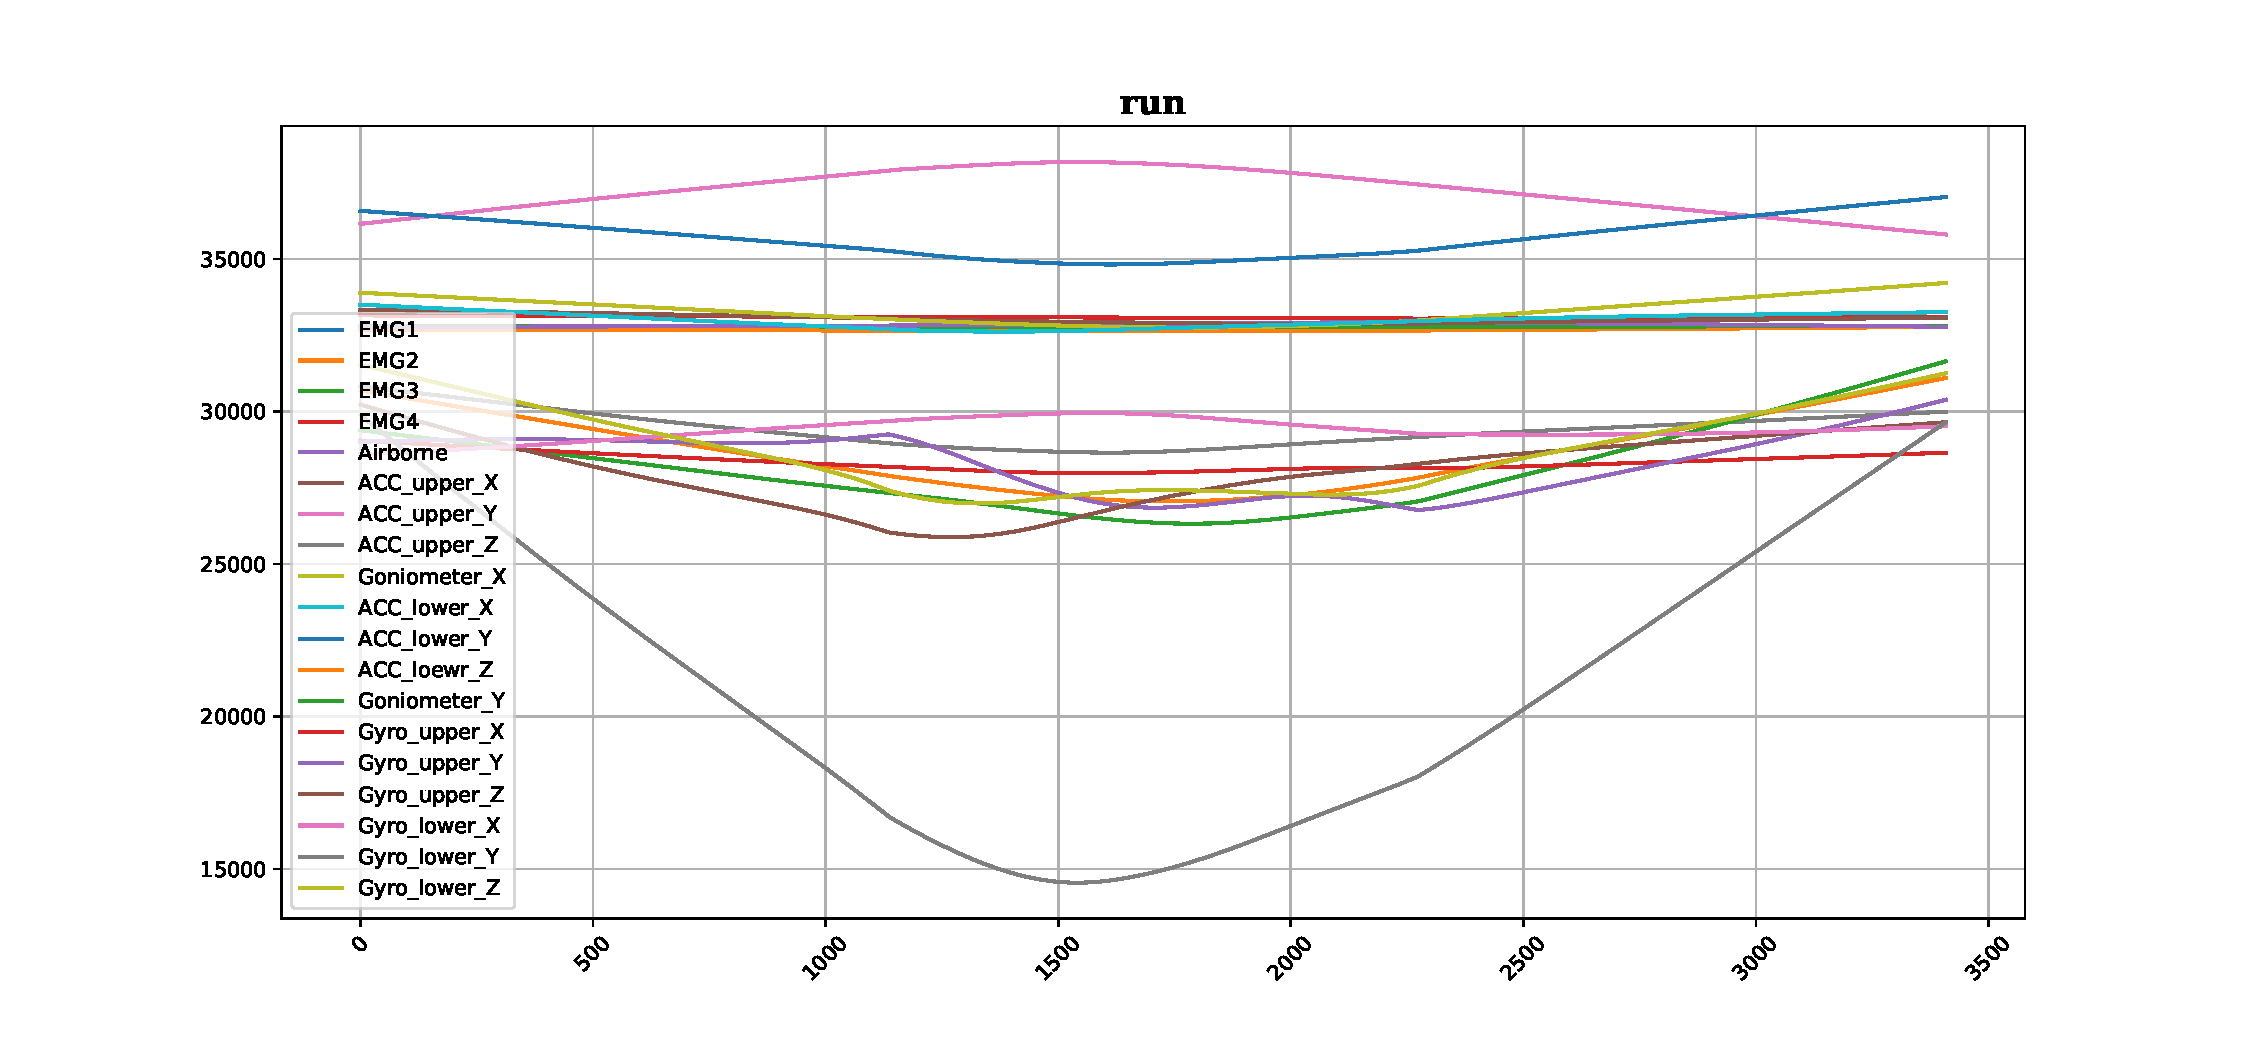
\includegraphics[width=\textwidth]{images/run_example.pdf}
		\caption{run}
	\end{minipage}
\end{figure}



\begin{figure}[!tbp]
	\begin{minipage}[b]{0.31\textwidth}
		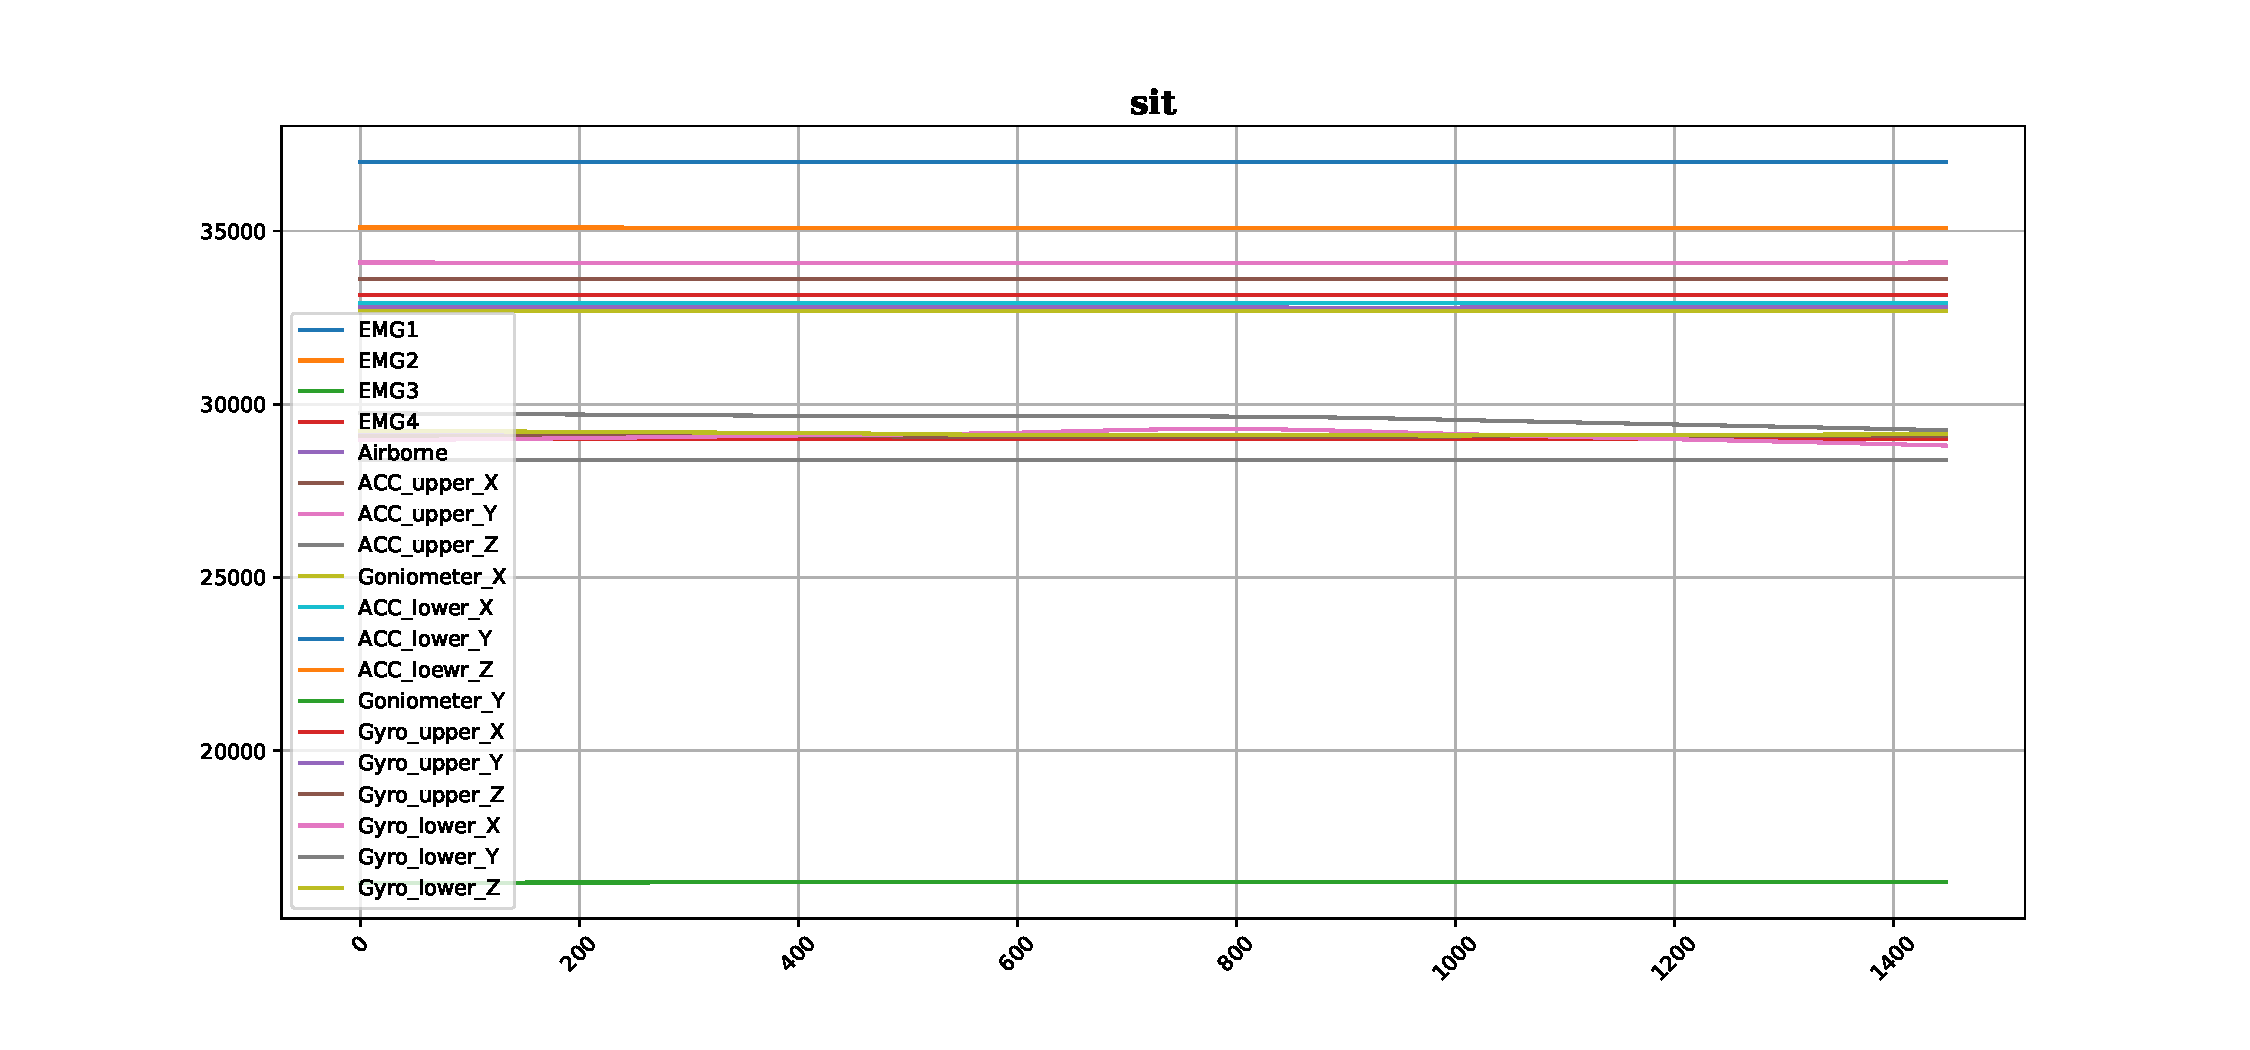
\includegraphics[width=\textwidth]{images/sit_example.pdf}
		\caption{sit}
		\label{sit}
	\end{minipage}
	\begin{minipage}[b]{0.31\textwidth}
		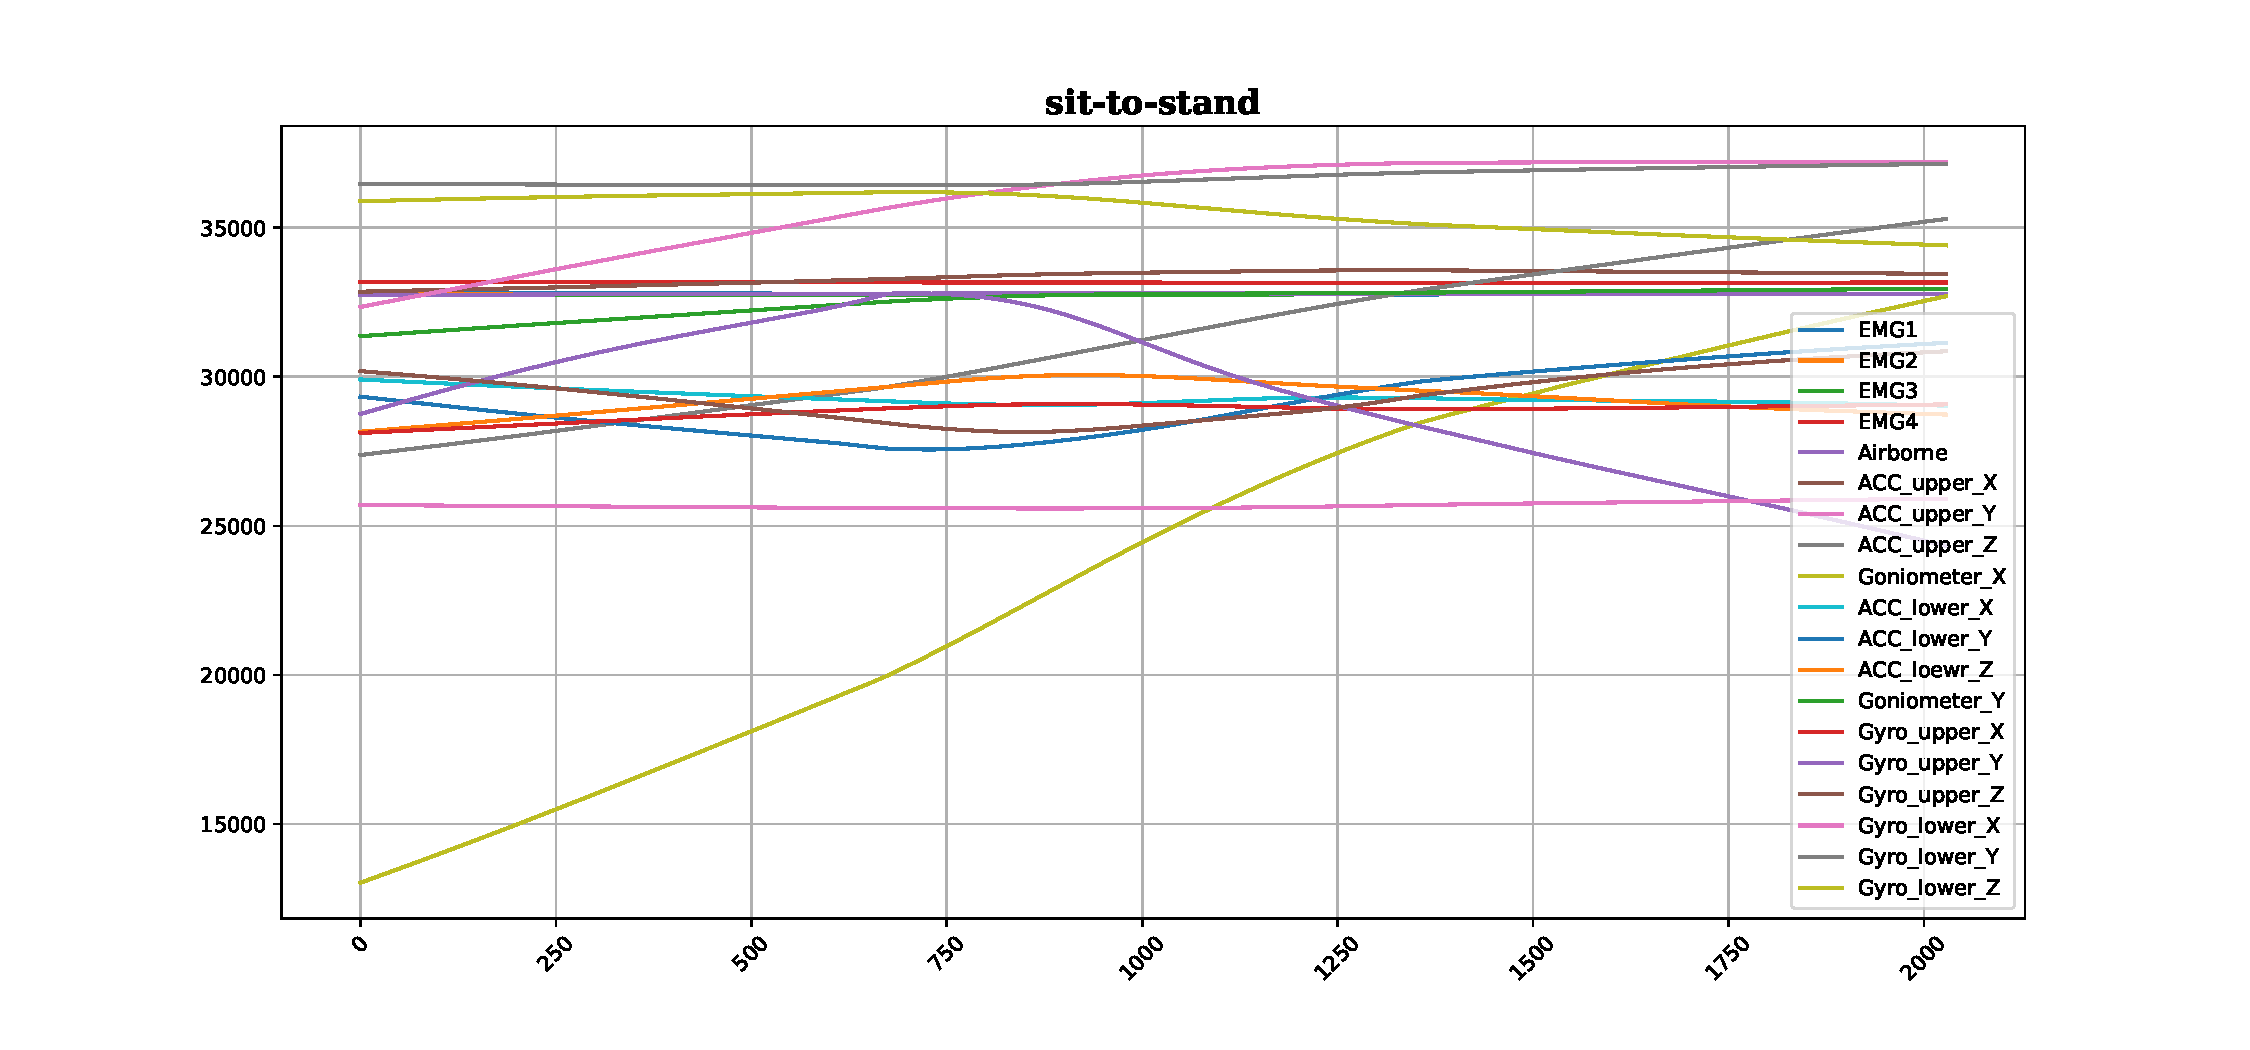
\includegraphics[width=\textwidth]{images/sit-to-stand_example.pdf}
		\caption{sit-to-stand}
	\end{minipage}
	\begin{minipage}[b]{0.31\textwidth}
		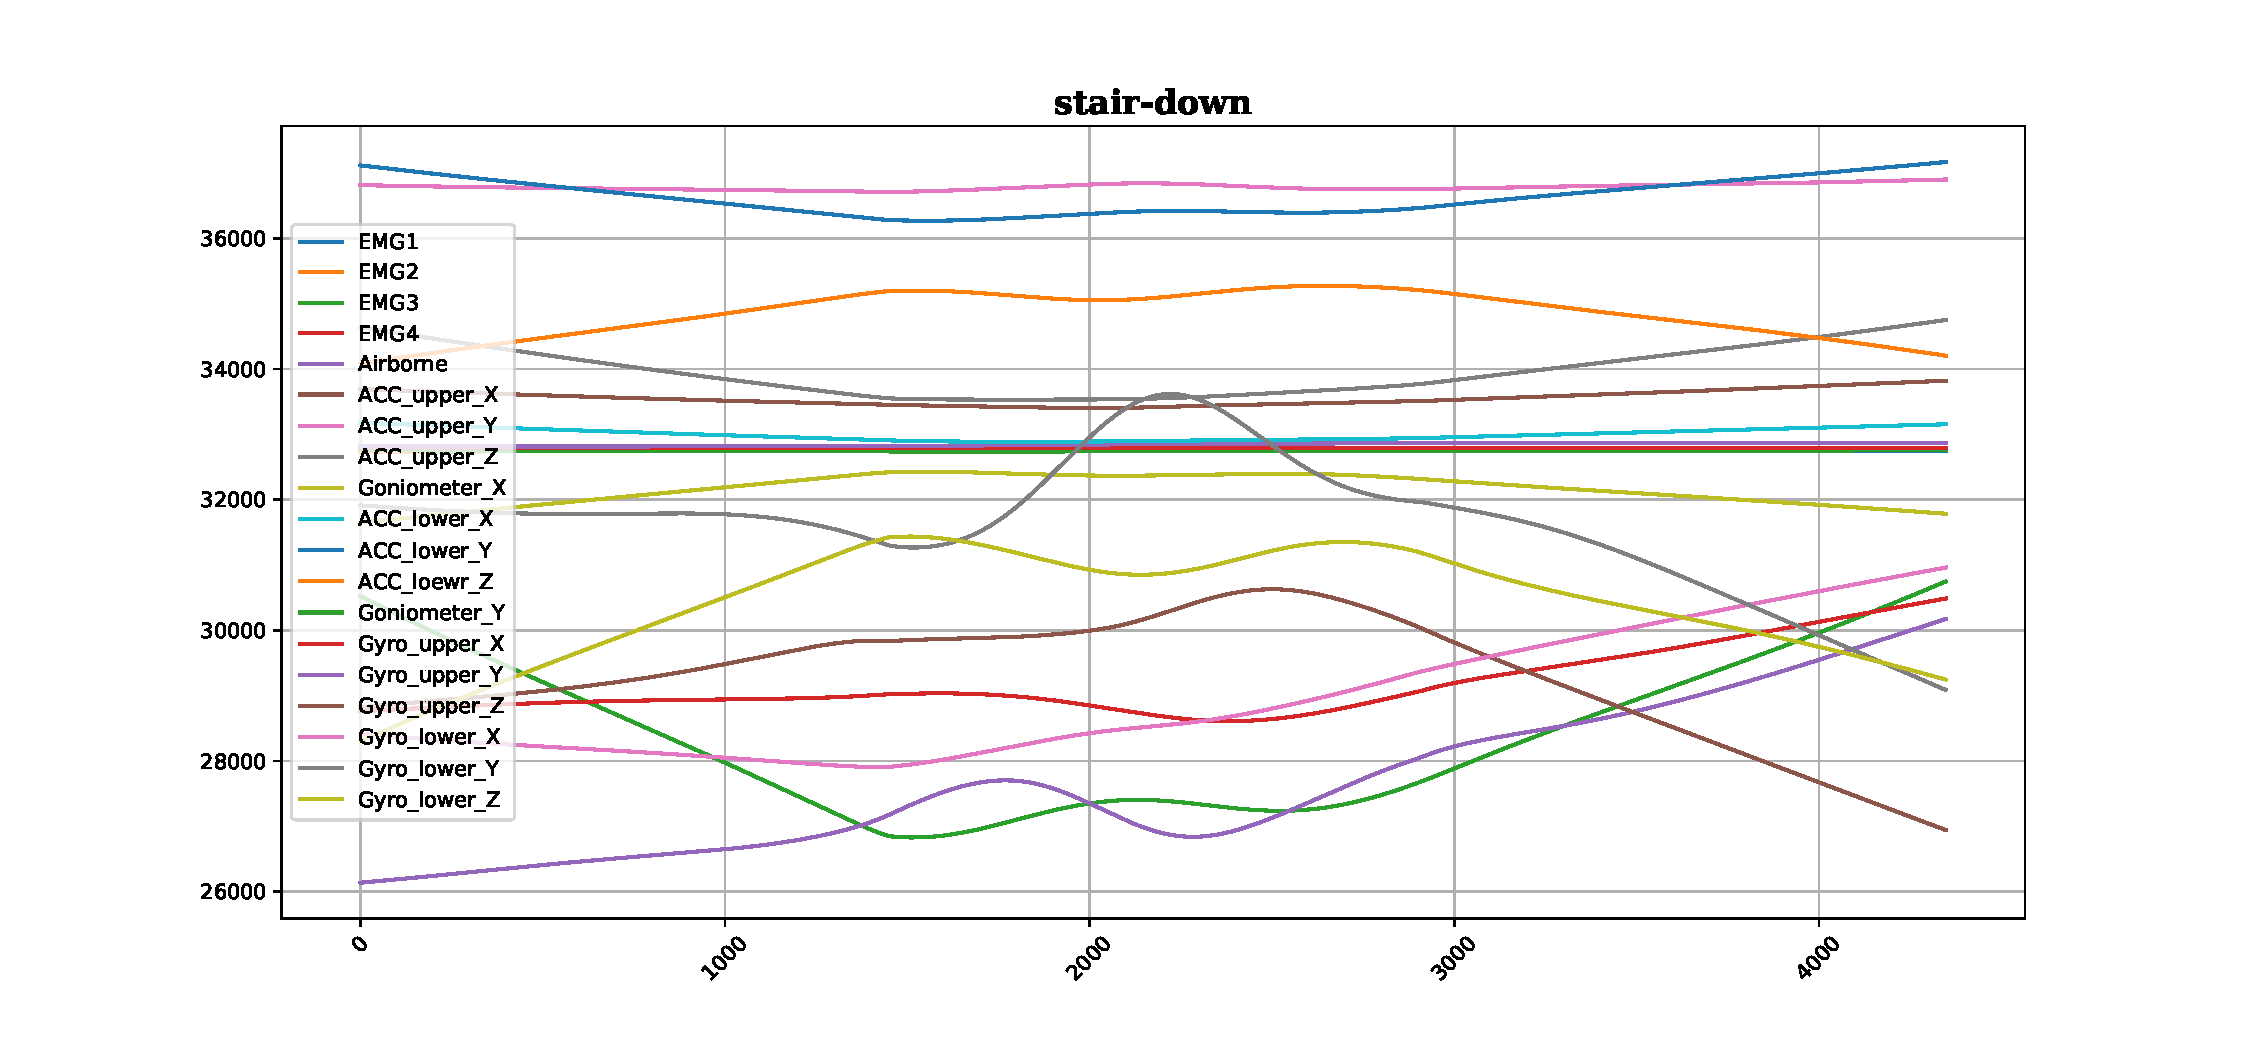
\includegraphics[width=\textwidth]{images/stair-down_example.pdf}
		\caption{stair-down}
	\end{minipage}
\end{figure}


\begin{figure}[!tbp]
	\begin{minipage}[b]{0.31\textwidth}
		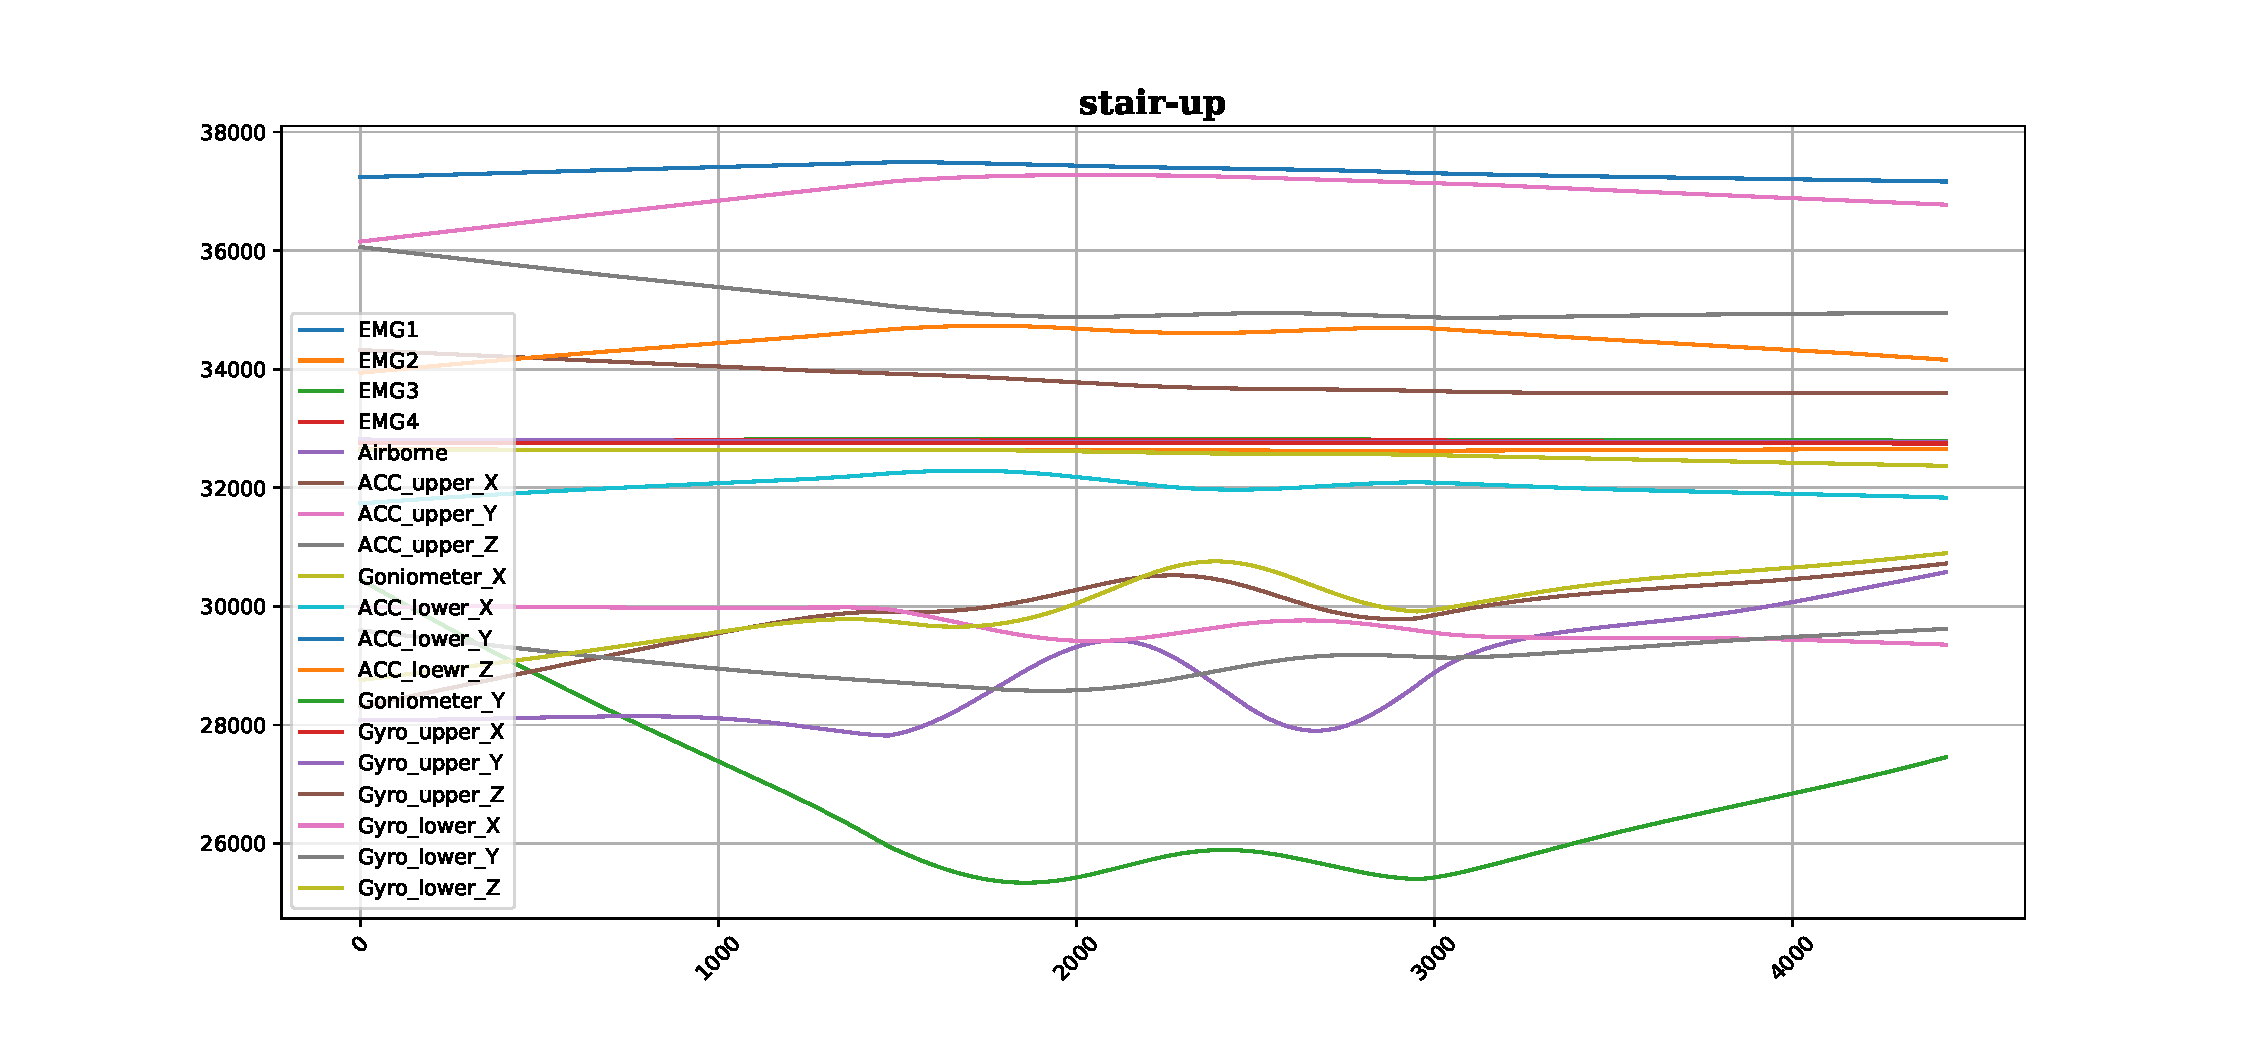
\includegraphics[width=\textwidth]{images/stair-up_example.pdf}
		\caption{stair-up}
	\end{minipage}
	\begin{minipage}[b]{0.31\textwidth}
		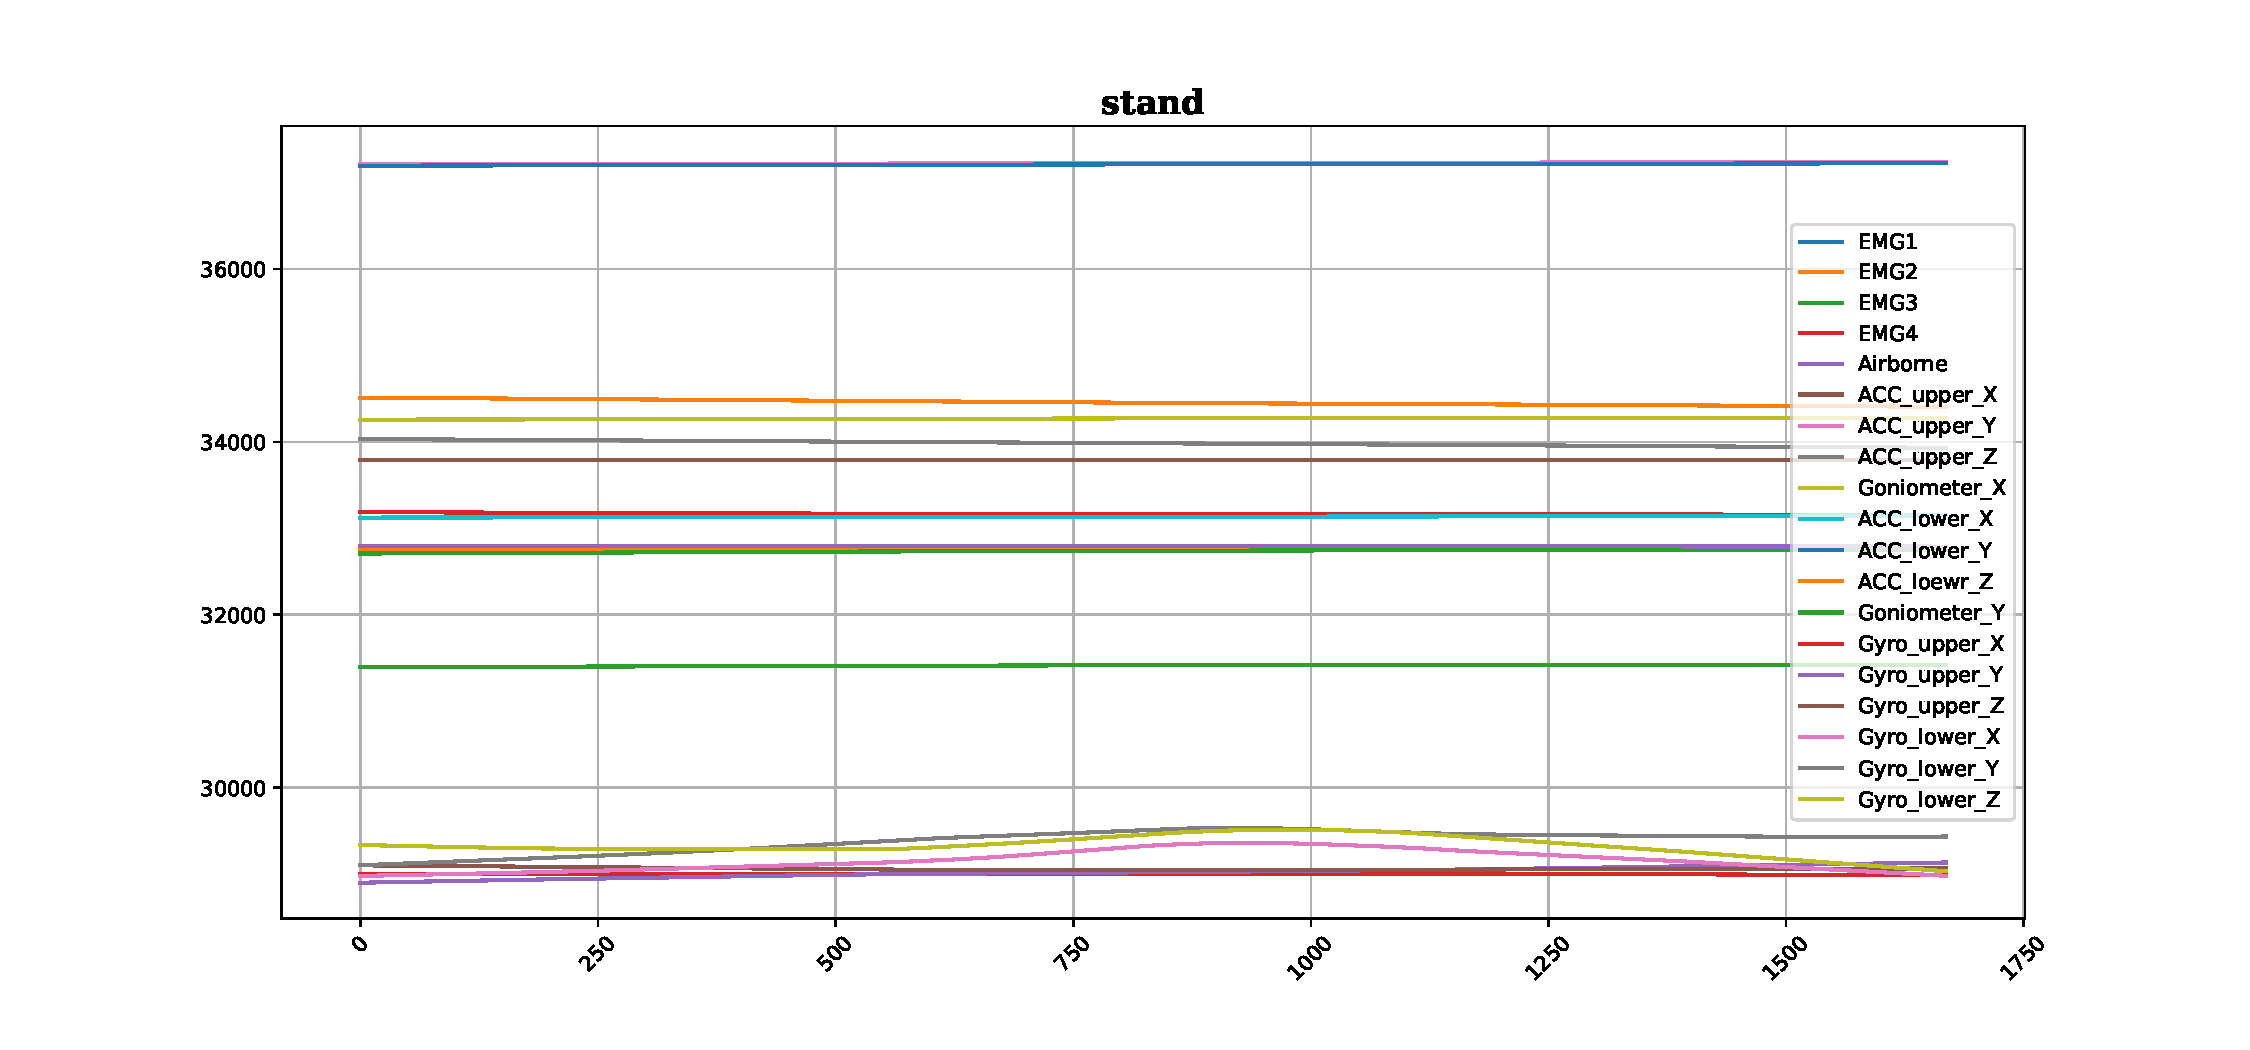
\includegraphics[width=\textwidth]{images/stand_example.pdf}
		\caption{stand}
		\label{stand}
	\end{minipage}
	\begin{minipage}[b]{0.31\textwidth}
		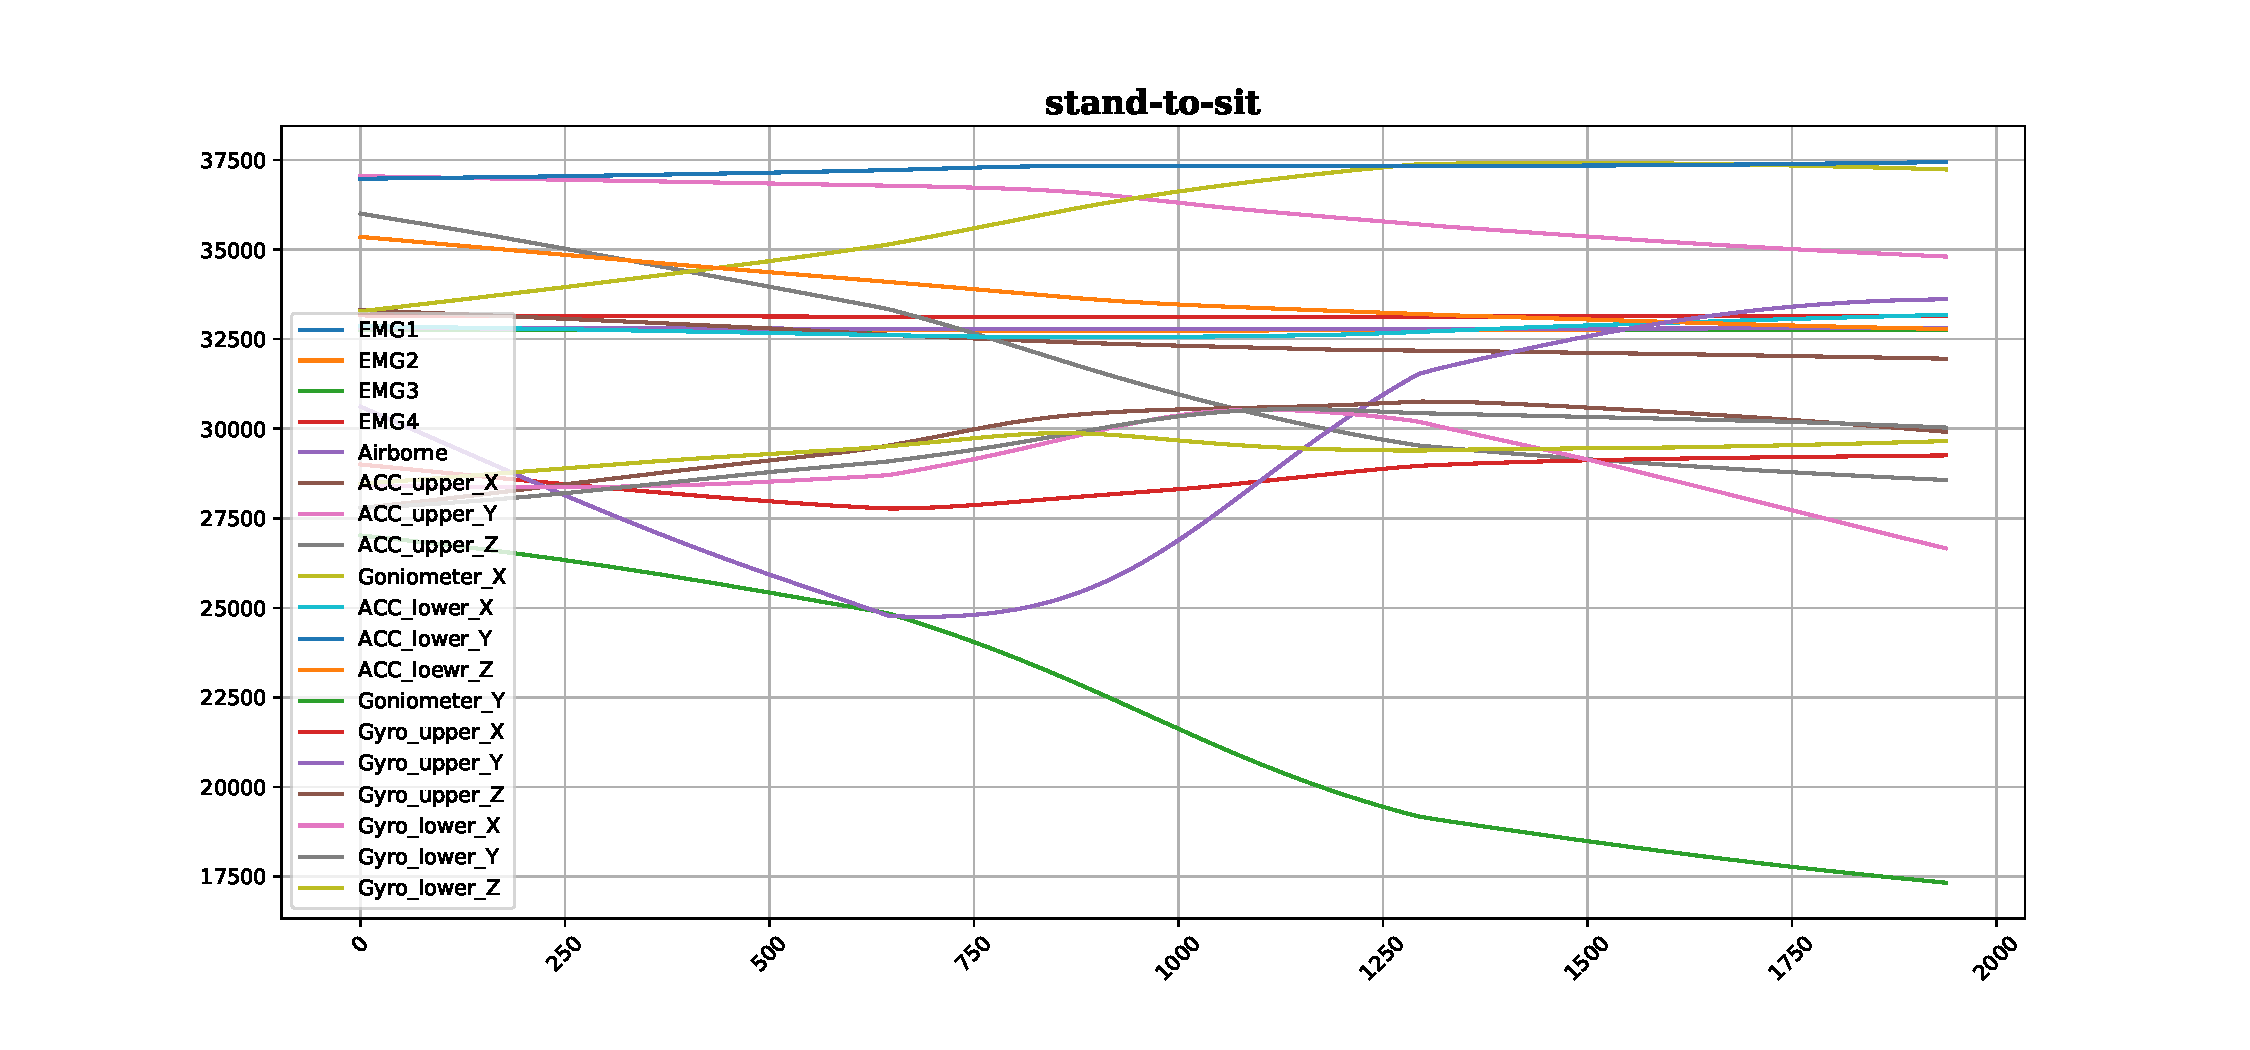
\includegraphics[width=\textwidth]{images/stand-to-sit_example.pdf}
		\caption{stand-to-sit}
	\end{minipage}
\end{figure}

\begin{figure}[!tbp]
	\begin{minipage}[b]{0.31\textwidth}
		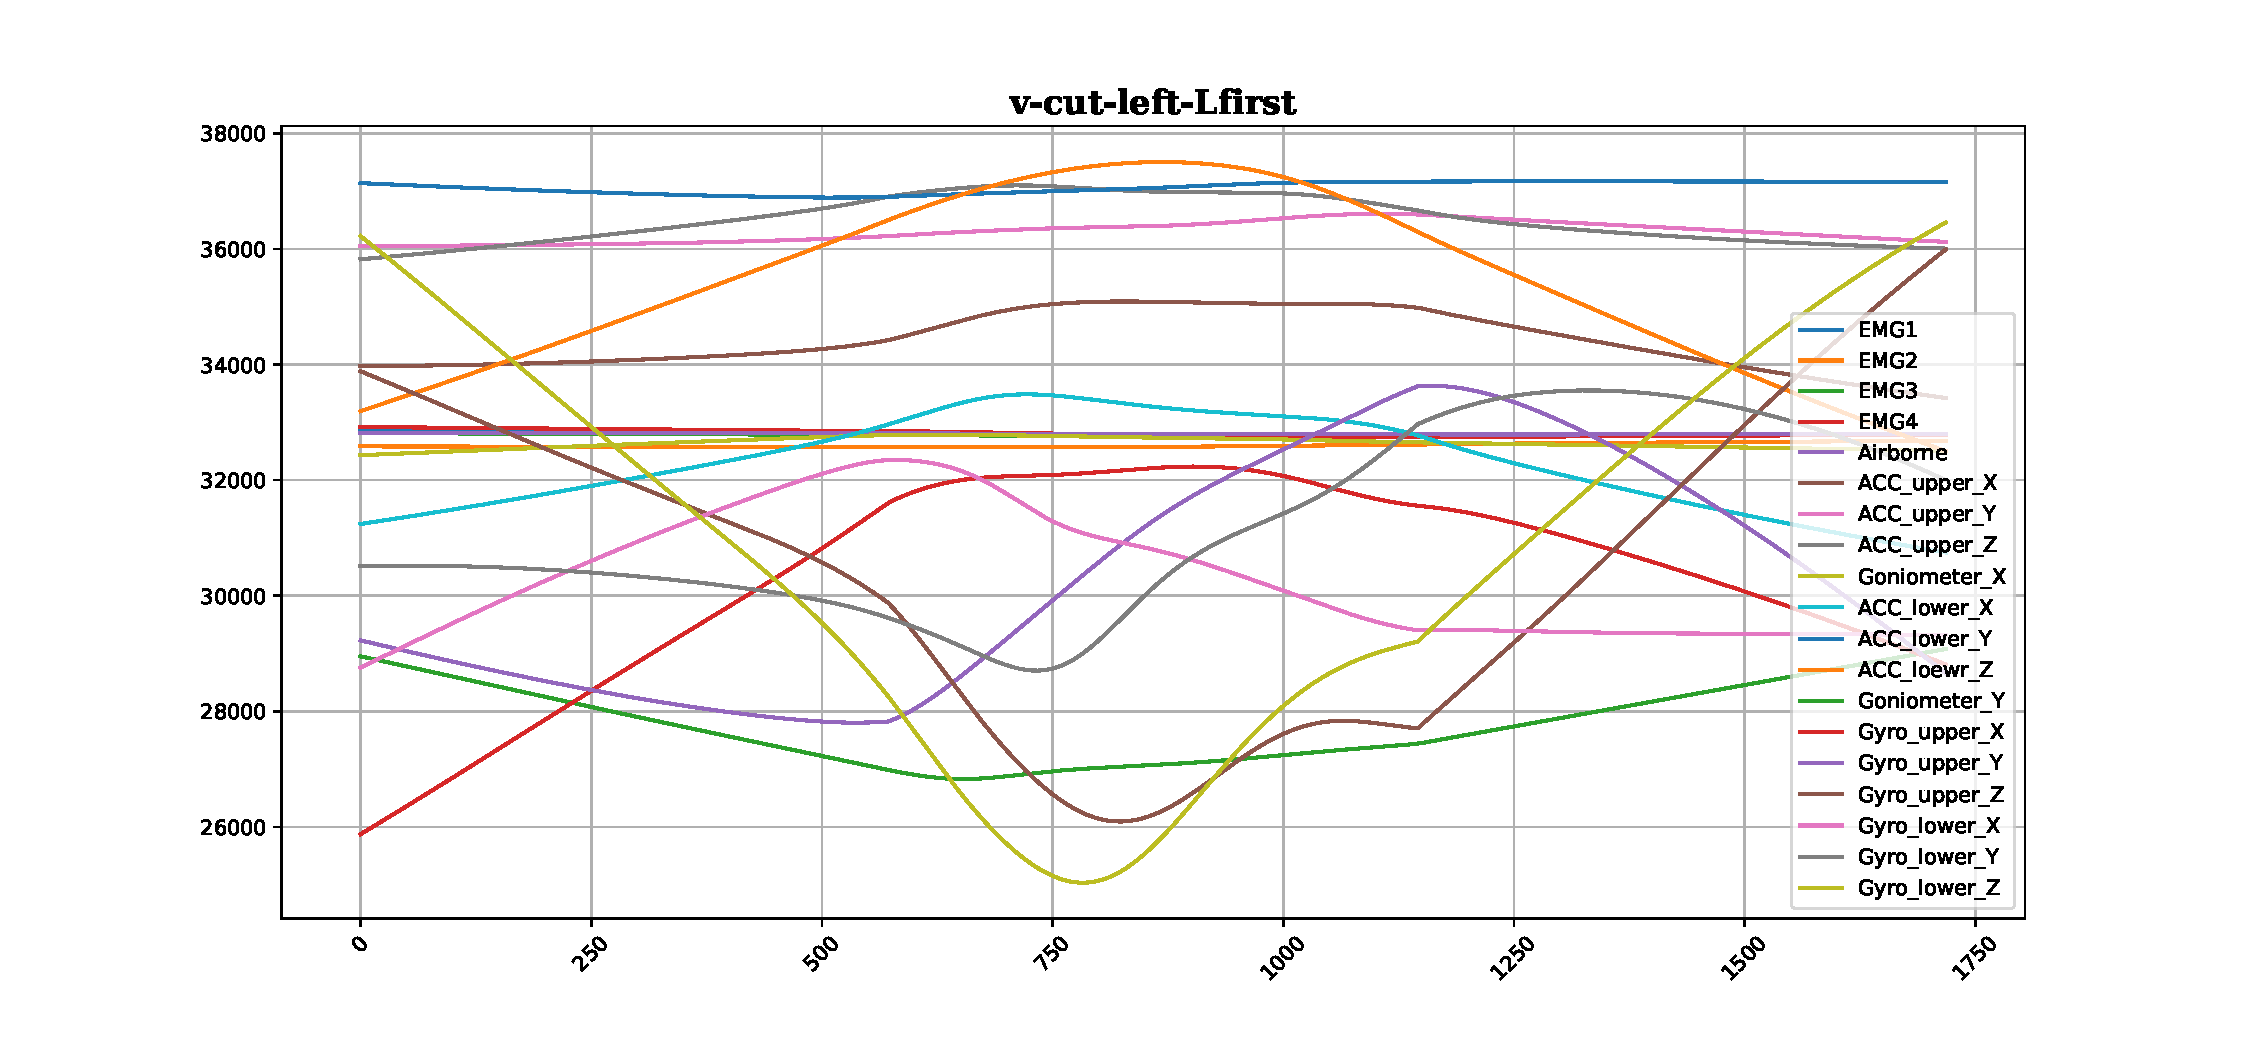
\includegraphics[width=\textwidth]{images/v-cut-left-Lfirst_example.pdf}
		\caption{v-cut-left-Lfirst}
	\end{minipage}
	\begin{minipage}[b]{0.31\textwidth}
		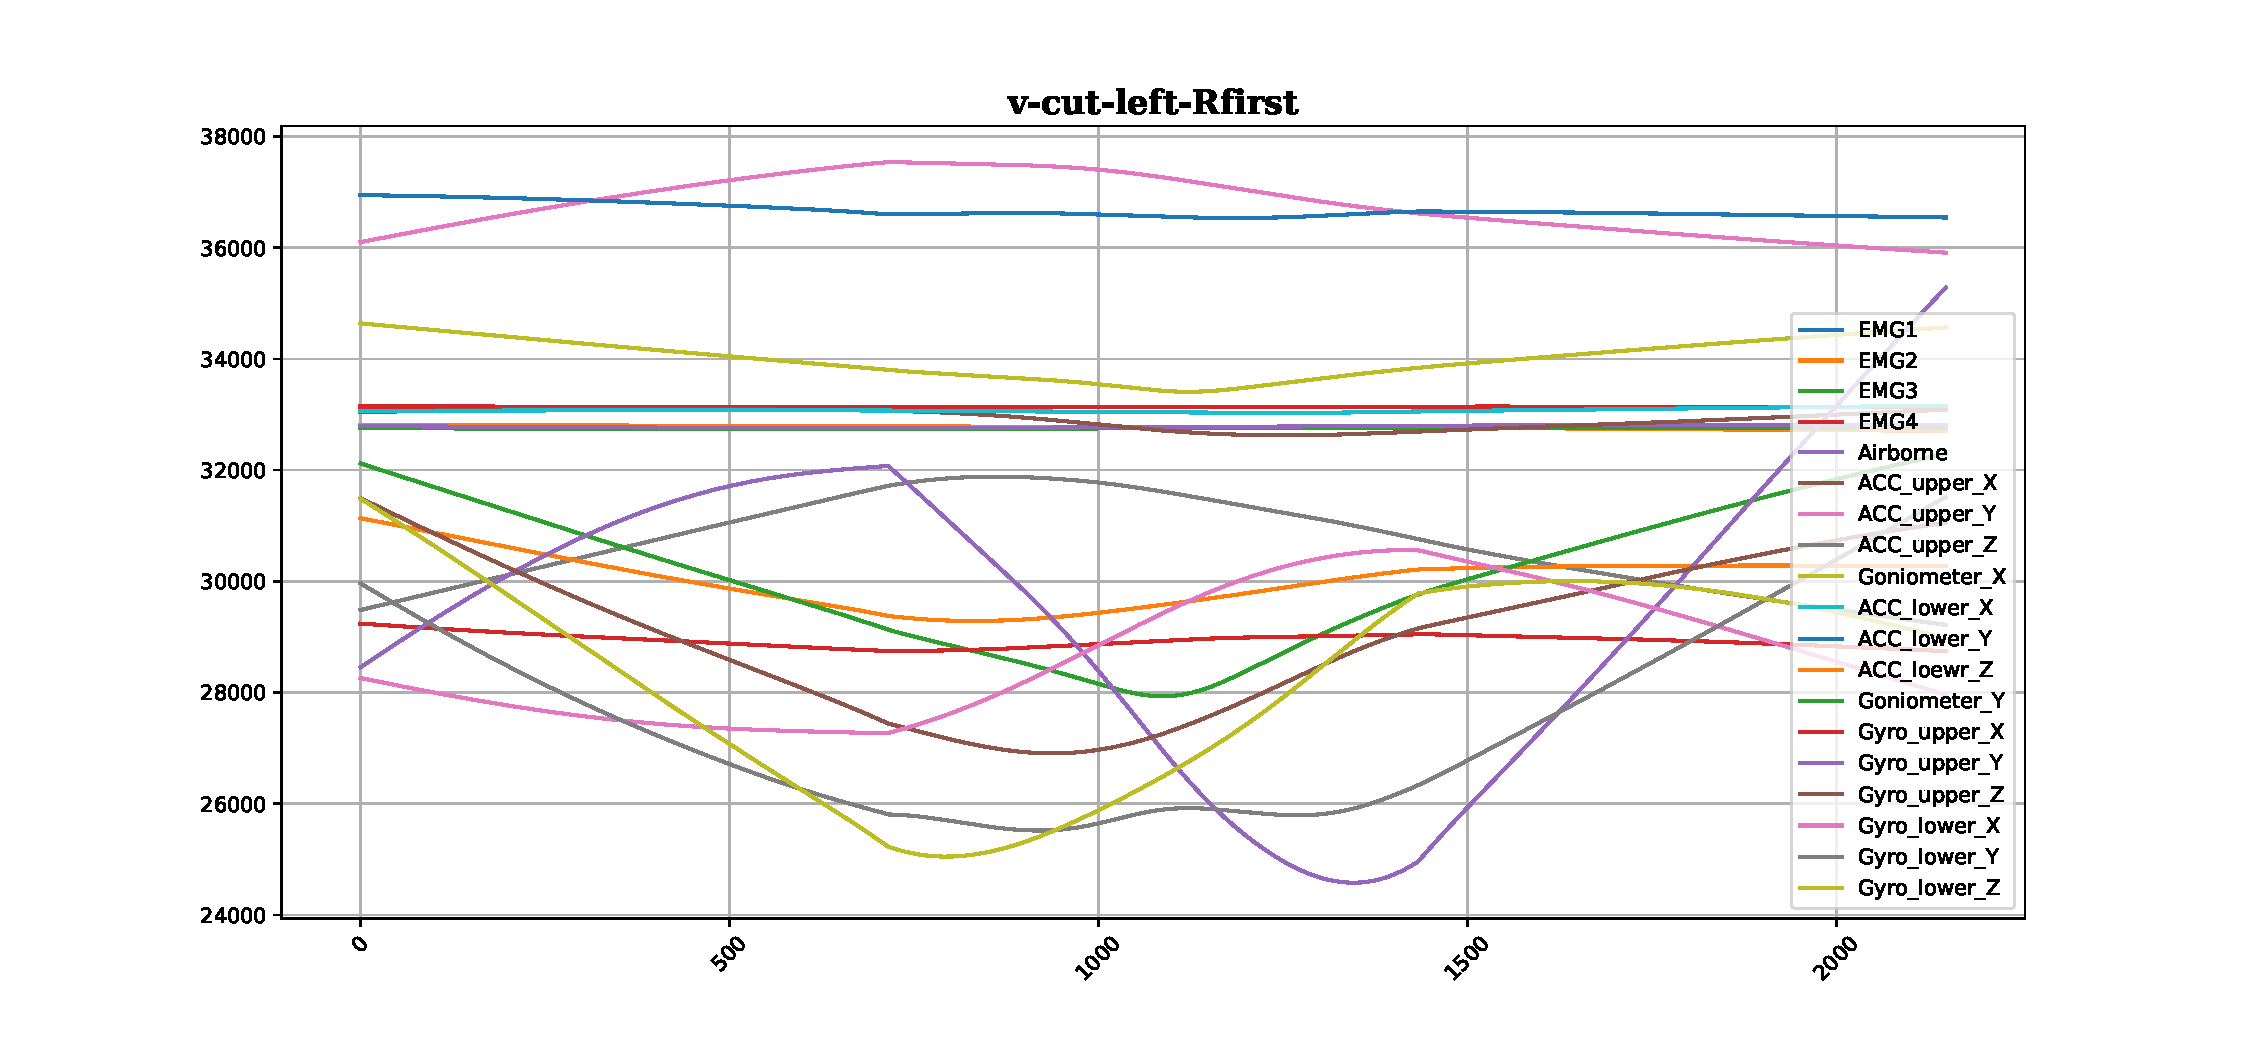
\includegraphics[width=\textwidth]{images/v-cut-left-Rfirst_example.pdf}
		\caption{v-cut-left-Rfirst}
	\end{minipage}
	\begin{minipage}[b]{0.31\textwidth}
		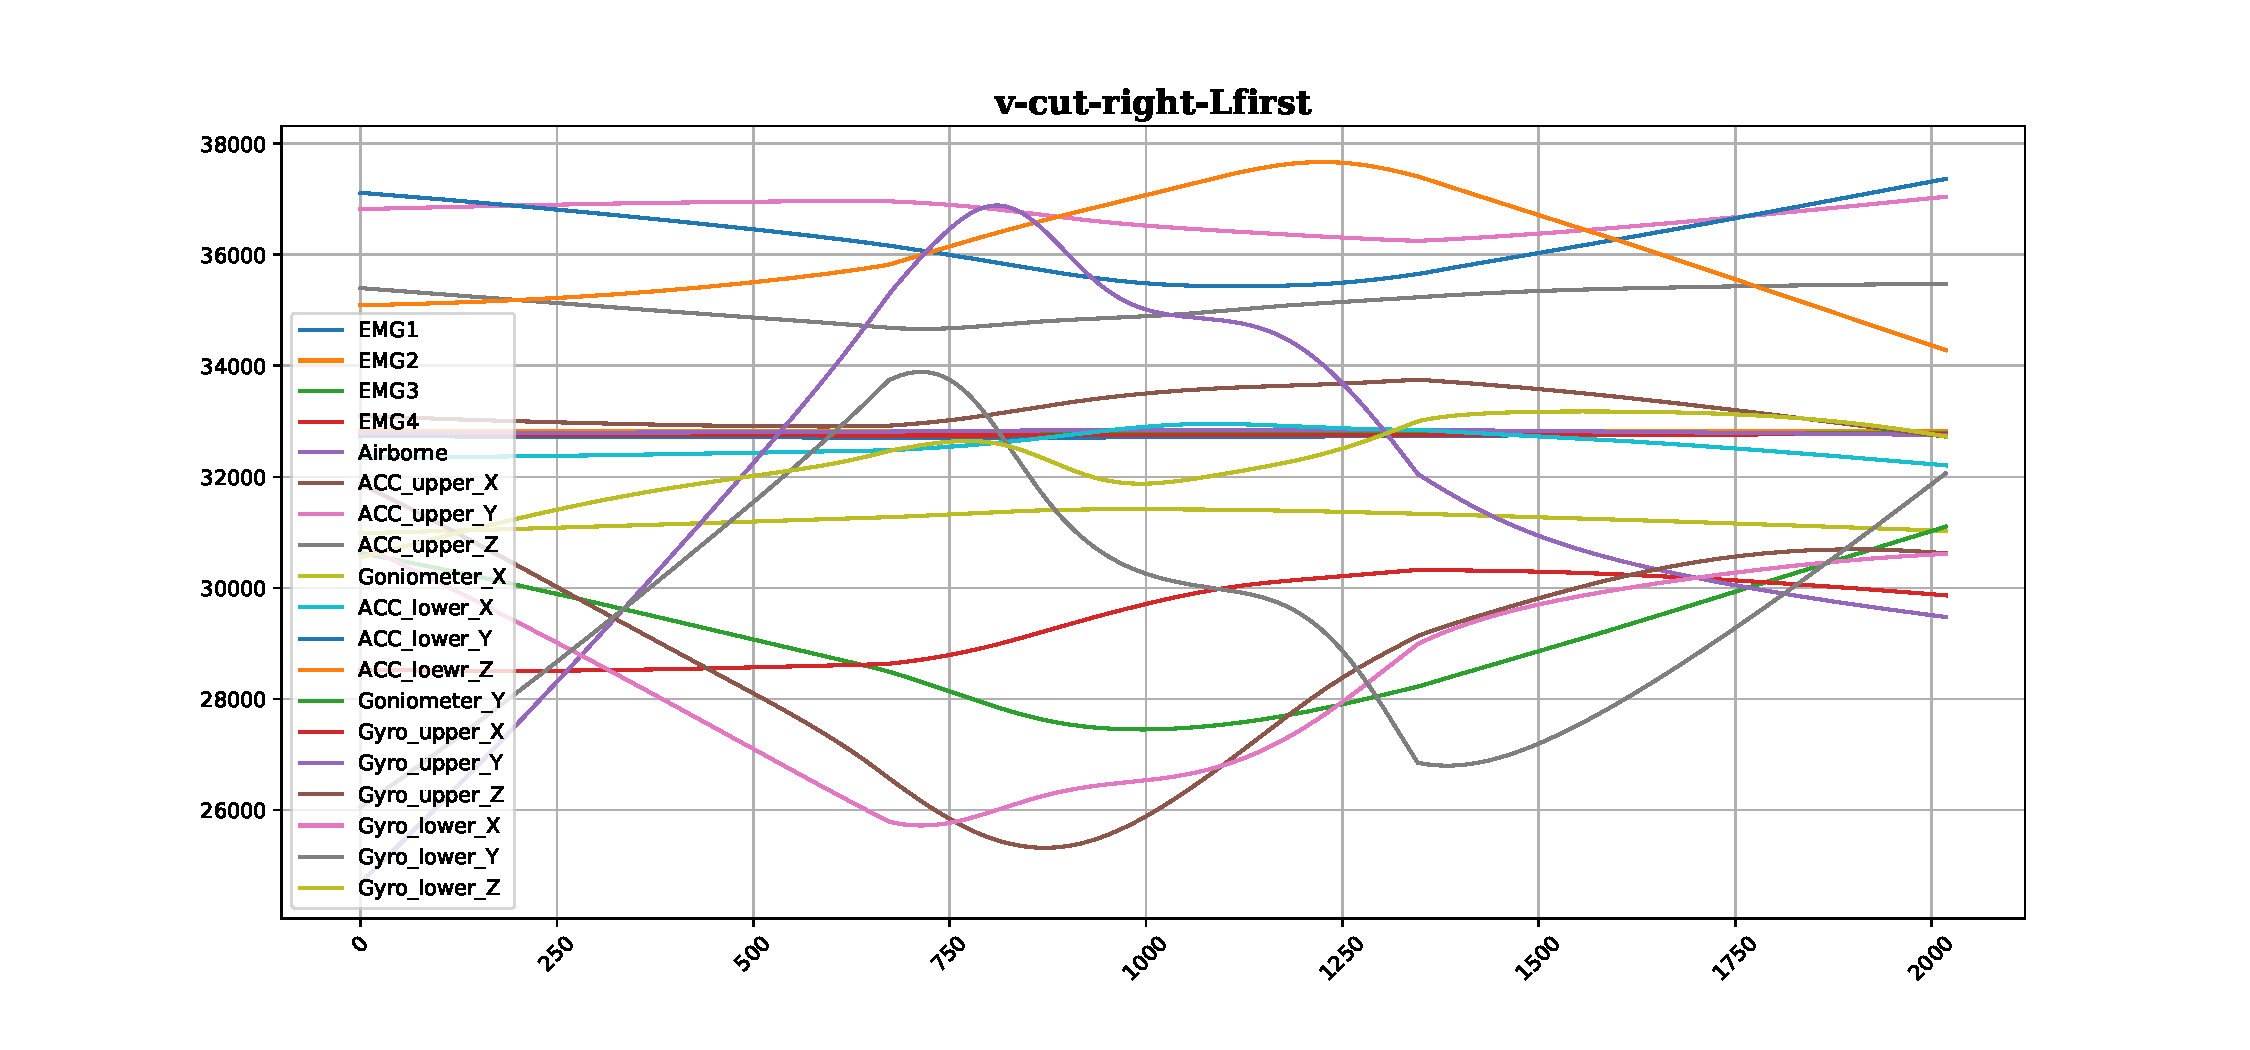
\includegraphics[width=\textwidth]{images/v-cut-right-Lfirst_example.pdf}
		\caption{v-cut-right-Lfirst}
	\end{minipage}
\end{figure}


\begin{figure}[!tbp]
	\begin{minipage}[b]{0.45\textwidth}
		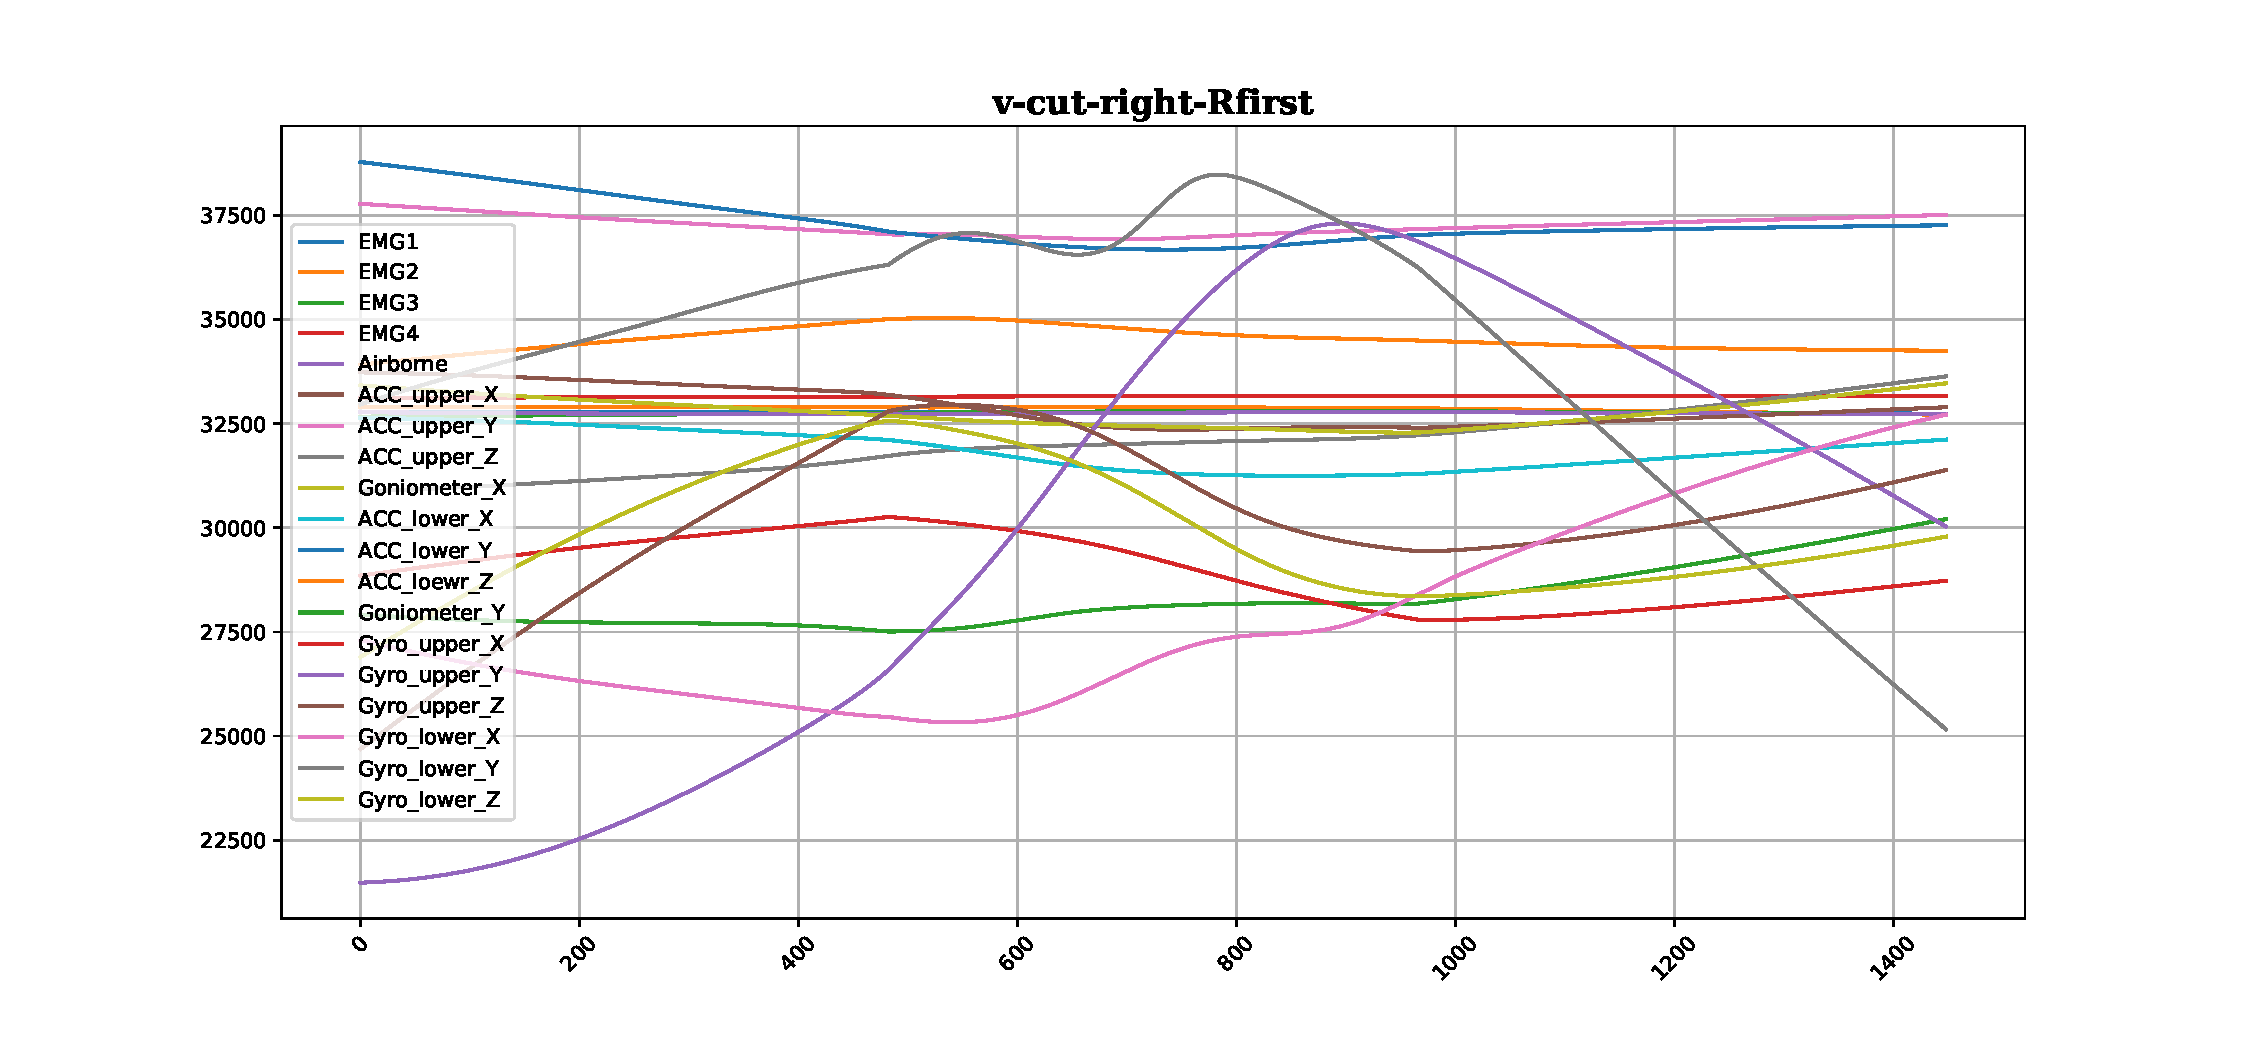
\includegraphics[width=\textwidth]{images/v-cut-right-Rfirst_example.pdf}
		\caption{v-cut-right-Rfirst}
	\end{minipage}
	\begin{minipage}[b]{0.45\textwidth}
		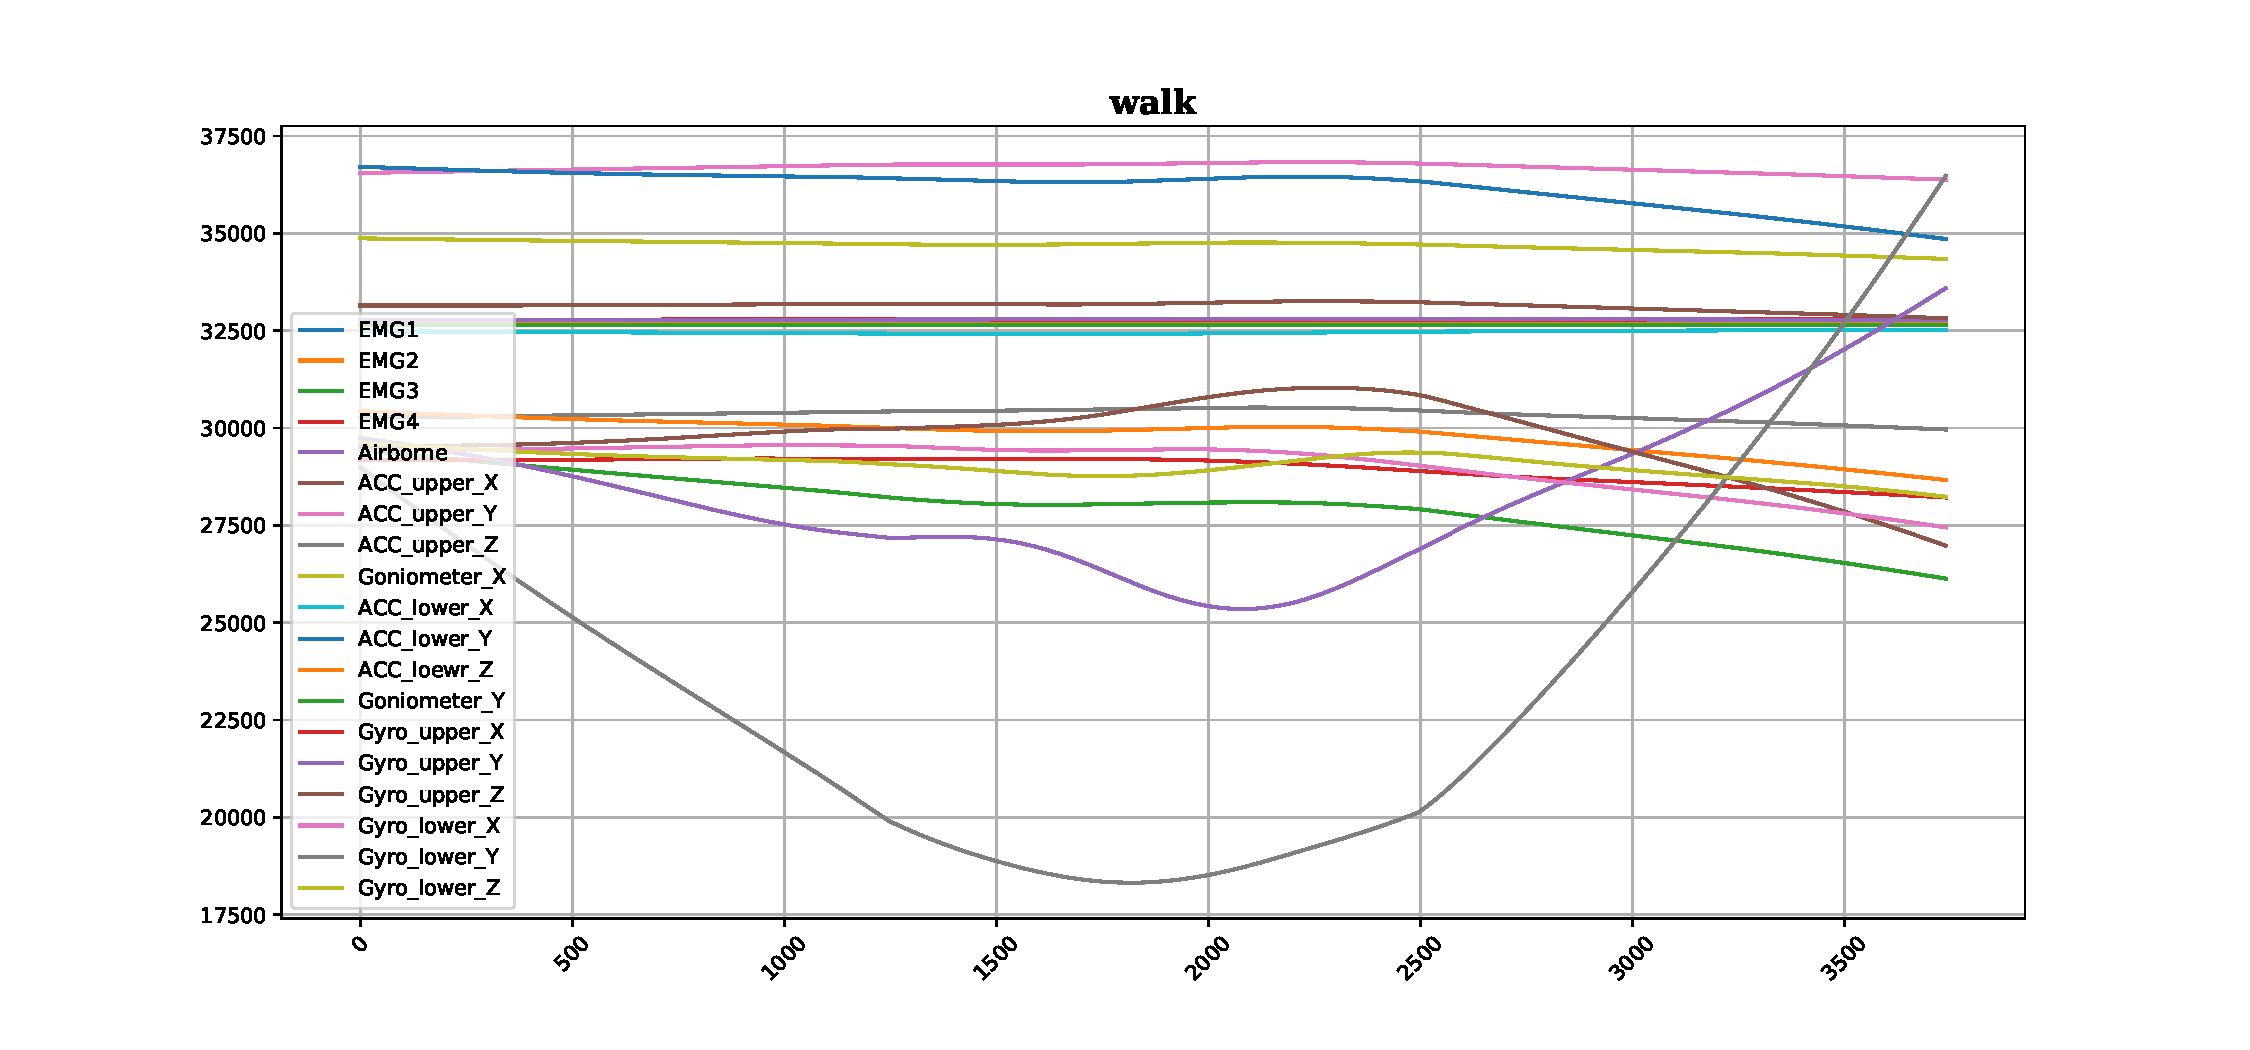
\includegraphics[width=\textwidth]{images/walk_example.pdf}
		\caption{walk}
		\label{sm22}
	\end{minipage}
\end{figure}



\section{Data Analysis}


\subsection{Data Analysis with $\mathcal{P}(\Theta_{1})$}
The last procedure to complete the full scheme in Figure \ref{dig:p1} is the implementation of the
\emph{Fully-Connected Neural Network (FCNN)}. Applying this \emph{Deep Learning} approach on the preprocessed
data serves as an alternate technique to optmize the loss function and increase accuracy.

When implementing FCNN using \emph{Pandas} \cite{pandasdataframe} and \emph{Scikit-Learn} \cite{scikitlearn}, there are several specifications to account for. Among them figure the
\emph{activation function}, the regularization factor \emph{alpha}, and the number of neurons per $ith$ hidden layer. To briefly
summarize some parameters, as per relevance or rule of thumbs, we describe their optional values:
\begin{itemize}
    \item The solver for the weight optimization ('lbfgs', 'sgd', 'adam')
    \item The size of hidden units ranging between $100 \pm 20$ for $ith$ hidden layer
    \item The regularization factor varying between $0.1$ and $0.00001$\footnote{Practice shows that
    by varying alpha the classifier has greater chance to perform way better than by adjusting the
    number of units per layer, or trying other algorithms.}
    \item The activation function for the hidden layers ('identity', 'logistic', 'tanh', 'relu')
\end{itemize}

Given the preprocessed data, whose order of magnitude scales to 1000+ data points, the default parameters
reveal themselves ideal to test out first. Then, based on the obtained results, we would assess the accuracy of
the prediction by tuning the other parameters (e.g. alpha) accordingly with the expectations of optimizing
the classifier and improving the accuracy.

The settings for the default values when running the MLPClassifier are: % source: \parencite{sklearnMLPclassifier}
\begin{center}
    \begin{tabular}{ c c c c c }
    \textbf{Solver} & \textbf{Activation Function} & \textbf{Hidden Units}  &  \textbf{Alpha} \\
    \textit{lbfgs} & \textit{relu} & \textit{50} & \textit{0.01} \\
    \end{tabular}
\end{center}
Surprisingly, both the training and testing errors score an error rate of $83.7\%$. Hoping
to find the parameters that work best for the task optimization, we performed \emph{Grid Search} by combining
above-mentioned options and tweaking them in the same range as in our first test. For instance, the chosen
values for alpha were $10^{-1}, 10^{-2}, 10^{-3}, 10^{-4}$, and $10^{-5}$.

Finally, the best parameters set found on the classifier development set are:
\begin{center}
    \begin{tabular}{ c c c c c }
    \textbf{Solver} & \textbf{Activation Function} & \textbf{Hidden Units}  &  \textbf{Alpha} \\
    \textit{lbfgs} & \textit{tanh} & \textit{20} & \textit{0.01} \\
    \end{tabular}
\end{center}
with an improved accuracy of $84.44\%$.

\subsection{Data Analysis with $\mathcal{P}(\Theta_{2})$}

Giving that the same $Stastistical_{Technique}$, namely \emph{Fully-Connected Neural Network (FCNN)} was used for  $\mathcal{P}(\Theta_{2})$ the prior section parameters definitions holds the same however, instead of using \emph{Scikit-Learn} we set up an environment where the \emph{FCNN} algorithm was implemented using \emph{keras} with \emph{Tensor-flow} back-end for \emph{gpu} usage.

\subsubsection{Experimental Setup}
Train an \emph{FCNN} with such high dimension dataset $D$ $[6401 \times 153]$ is computationally expensive(in fact this is the reason we were force to used \emph{keras}) so trying a \emph{cross-validation} plus  \emph{grid-search} as in   $\mathcal{P}(\Theta_{1})$ is not piratically possible. We used instead a simply $75\%$ and $25\%$ train-test split, and randomly tested different \emph{FCNN} architectures. We also min-max scale so that \emph{FCNN} was trained using features $\in [0,1]$ interval, for increasing the convergence time.



\section{Results and Discussions}

\subsection{Results and Discussions for  $\mathcal{P}(\Theta_{2})$}

\begin{table}[h!]
	\begin{center}
		\begin{tabular}{||c c c c c c c||}
			\hline
			$H_{L1}(H_{units},fun)$&$H_{L2}$&$H_{L2}$& $\alpha$ & $Train_{Score}$ & $Test_{Score}$  & $Challenge_{score}$  \\ [0.5ex]
			\hline
			60,relu
			&
			87,tanh
			&
			23, sigmoid
			&0.000001& $95\%$ & $91\%$ & $64\%$  \\
			\hline
		\end{tabular}
		\caption{Resuts on $\mathcal{P}(\Theta_{2})$}
		\label{table:p2_result}
	\end{center}
\end{table}

\begin{figure}[htpb!]
	\centering
	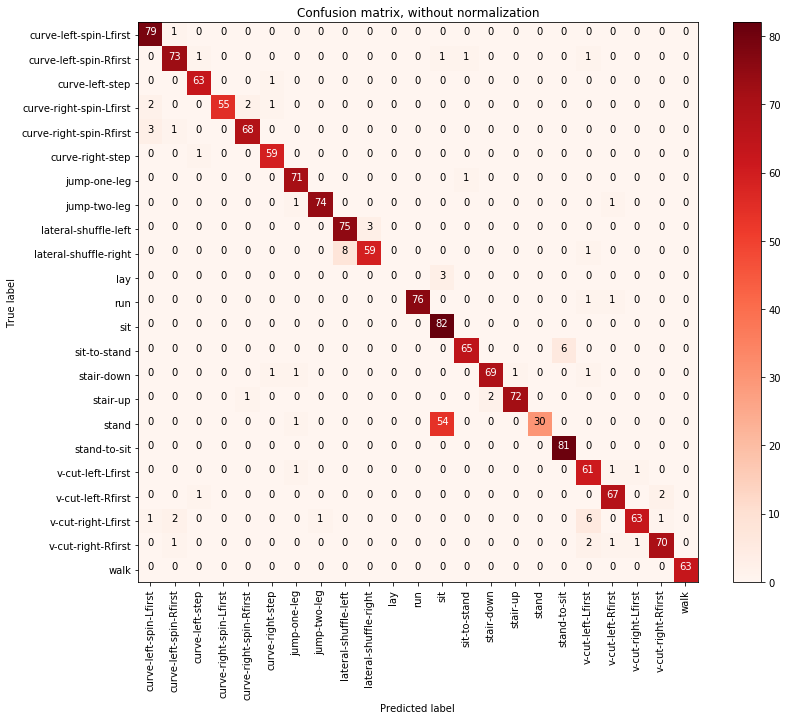
\includegraphics[width=\textwidth]{images/conf_ma.png}
	\caption{$\mathcal{P}(\Theta_{2})$  Confusion matrix on test data.}
	\label{fig:confusion}
\end{figure}


From Figure \ref{fig:confusion} we can conclude that the most misclassification occurs with the classes \emph{stand} and \emph{sit} which intuitively are mechanically similar, this can be further confirmed by looking at the smoothen ($\mu$) plots \ref{sit} and \ref{stand}. We tried to modified the $Preprocessing_{ \ method \ 1}$ to include some manually crafted features that will indicate a clear different between \emph{stand} and \emph{sit}, they can be summarized as follows:


\begin{itemize}
	\item The first and second derivate of $\mu$, since we believed the direction of the movement had to be different.
	\item The maximum value of the $\mu$, since sensor data related to distance from the floor must different for both classes.
	\item increase to 5 five the number of statistical moments.
\end{itemize}

Unfortunately none of them gave better results on the test data. The main reason being that this particular adjustment had to me made to all the features, this in term caused other features to get noise, as a result, the decrease in misclassification gained in the pair  \emph{stand}, \emph{sit} was undermined by the increase of misclassification on other features, particularly \emph{sit-to-stand} and \emph{stand-to-sit}.

\subsection{Results and Discussions for  $\mathcal{P}(\Theta_{1})$}

In Table \ref{table:p1_result} we can observe that the Challenge score is inferior to that reached on $\mathcal{P}(\Theta_{2})$, since this was the case, we focused our efforts of optimization on $\mathcal{P}(\Theta_{2})$.

\begin{table}[h!]
	\begin{center}
		\begin{tabular}{||c c c c c c||}
			\hline
			$H_{units}$ &Activation function & $\alpha$ & $CV_{train}$ & $CV_{test}$  & Challenge score \\ [0.5ex]
			\hline
			20 & tanh &0.01& (??) & $84.44\%$& $54\%$  \\
			\hline
		\end{tabular}
		\caption{Resuts on $\mathcal{P}(\Theta_{1})$}
		\label{table:p1_result}
	\end{center}
\end{table}

\section{Conclusion}

\subsection{Conclusion for $\mathcal{P}(\Theta_{1})$}

\begin{itemize}
	\item In retrospective we realized that we introduced some \emph{data leakage} on this implementation, since while constructing $PCA_{|class}$ we feed the algorithms the whole dataset. This could be an explanation for the difference in performance on our $CV_{test}$ and challenge score.
	\item In $Preprocessing_{ \ method \ 1}$  we arbitrarily choose the number of time steps to be 56810 per signal, we believed that this decision should be made with more empirical knowledge of the phenomena, to increase the performance of $\mathcal{P}(\Theta_{1})$.
	\item We also implemented \emph{Boosting} with \emph{random forest} with $4\%$ increase in $CV_{test}$ however, the competition had already finished and we could not test the result on the challenge data.
\end{itemize}

\subsection{Conclusion for $\mathcal{P}(\Theta_{2})$}

\begin{itemize}
	\item After the competition finished we realized that one reason for the difference in performance between our test and the challenge score might have been that the splitting of our data was done randomly, we believe that setting aside entire subjects would have been a better approach, after all, an individual should walk and run in a similar manner.
	\item In other to increase the performance of $\mathcal{P}(\Theta_{2})$ we believe a window of sampling the signal $S_{data}$ should be implemented using expert knowledge on the subject. As a side note, we tried the latest by splitting $S_{data}$ into 3 sectors and then repeating $Preprocessing_{ \ method \ 2}$. unfortunately, this is very computational expensive, and the attempt, after days of running had to be stooped.

\end{itemize}

% \begin{thebibliography}{1}
% \bibitem{1}
% Cleveland, W.S. (1979) “Robust Locally Weighted Regression and Smoothing Scatterplots”. Journal of the American Statistical Association 74 (368): 829-836.

% \bibitem{2}
% Oraintara, S., Chen, Y. J., \& Nguyen, T. Q. (2002). Integer fast Fourier transform. IEEE Transactions on Signal Processing, 50(3), 607-618.

% \end{thebibliography}

% ==============================================================================
% START: Methods, Results, Discussions, Conclusion
% ==============================================================================